%!TEX TS-program = pdflatex
%!TEX encoding = UTF-8 Unicode
%!TEX root = 2020-04-04-papa-insinuarsi-nel-vuoto_libroA4_solofronte.tex

\documentclass[a4paper,
		       titlepage,
               headinclude,
               footinclude,
               BCOR5mm,
               numbers=noenddot,
               cleardoublepage=empty,
               tablecaptionabove,
               %twoside,
               %openright,
               openany
               ]{scrreprt}

\usepackage[T1]{fontenc}
\usepackage[utf8]{inputenc}

\usepackage[english,
            italian
            ]{babel}
            
\usepackage{amsmath,
		    amssymb}

\usepackage{indentfirst}

\usepackage[style=philosophy-modern,
            hyperref
            ]{biblatex}
            
\usepackage{chngpage}

\usepackage{calc}

\usepackage{listings}

\usepackage{graphicx}

\usepackage{epstopdf}

\usepackage{subfig}

\usepackage{lipsum}

\usepackage{shapepar}

\usepackage{pifont}

\usepackage[eulerchapternumbers,
            subfig,
            beramono,
            eulermath,
            pdfspacing,
            listings,
            dottedtoc
            ]{classicthesis}

\usepackage{arsclassica}

% ********************************************************************
% Personal commands
% ******************************************************************** 
\newcommand{\myName}{Michele Papa}
\newcommand{\myTitle}{Insinuarsi nel vuoto}
\newcommand{\mySubTitle}{Composizione in due varchi temporali}

\DeclareRobustCommand*{\clsname}[1]{{\normalfont\sffamily#1}}
\DeclareRobustCommand*{\pkgname}[1]{{\normalfont\sffamily#1}}
\DeclareRobustCommand*{\optname}[1]{{\normalfont\ttfamily#1}}
\DeclareRobustCommand*{\cmdname}[1]{\mbox{\lstinline[basicstyle=\normalsize\ttfamily]!\\#1!}}

\DeclareRobustCommand*{\classicthesis}{Classic\-Thesis}
\DeclareRobustCommand*{\arsclassica}{{\normalfont\sffamily ArsClassica}}


% ********************************************************************
% Hyper-references
% ******************************************************************** 
\newcommand{\mail}[1]{\href{mailto:#1}{\texttt{#1}}}


% ********************************************************************
% Graphics
% ********************************************************************
\graphicspath{{Graphics/}}


% ********************************************************************
% Code
% ********************************************************************
\definecolor{lightergray}{gray}{0.99}

\lstset{language=[LaTeX]Tex,
     keywordstyle=\color{RoyalBlue},
     basicstyle=\small\ttfamily,
     commentstyle=\color{Emerald}\ttfamily,
     stringstyle=\rmfamily,
     numberstyle=\scriptsize,
     showstringspaces=false,
     breaklines=true,
     frame=lines,
     backgroundcolor=\color{lightergray},
     flexiblecolumns=true,
     escapeinside={£*}{*£},
     firstnumber=last,
} 

\newcommand{\meta}[1]{$\langle${\normalfont\itshape#1}$\rangle$}

\lstset{	morekeywords=%
    {ProvidesPackage,RequirePackage,areaset,ifthenelse,%
     chapterNumber,undefined,boolean,DeclareRobustCommand,%
     spacedallcaps,textssc,MakeTextUppercase,lehead,%
     microtypesetup,textls,spacedlowsmallcaps,MakeTextLowercase,%
     sodef,allcapsspacing,lowsmallcapsspacing,thesection,%
     color,headmark,rohead,headfont,pnumfont,titleformat,%
     part,partname,thepart,chapter,thechapter,titlerule,%
     subsection,thesubsection,subsubsection,thesubsubsection,%
     paragraph,theparagraph,descriptionlabel,titlespacing,%
     formatchapter,textcolor,clearscrplain,rofoot,labelitemi,
     captionsetup,hypersetup}}

\lstnewenvironment{code}% 
   {\setkeys{lst}{columns=fullflexible,keepspaces=true}%
   \lstset{basicstyle=\small\ttfamily}}{}


% ********************************************************************
% Bibliography
% ******************************************************************** 
\bibliography{Bibliography}

\defbibheading{bibliography}{%
\cleardoublepage
\manualmark
\phantomsection
\addcontentsline{toc}{chapter}{\tocEntry{\bibname}}
\chapter*{\bibname\markboth{\spacedlowsmallcaps{\bibname}}
{\spacedlowsmallcaps{\bibname}}}}

\renewcommand*{\nameyeardelim}{\addcomma\space}

%-----------------------------------------------------------------------
%--------------------------------------------------- personalizzazioni -
%-----------------------------------------------------------------------

\usepackage{epigraph}

\usepackage{floatflt}

\usepackage{setspace}

%\linespread{1.1}

\usepackage{tikz}

\usepackage{color}

\usepackage{pdfpages} 

\usepackage{wrapfig} 

\usepackage{multirow}

\usepackage{booktabs}

\usepackage{tabularx}
%-----------------------------------------------------------------------
%----------------------------------------------------------- documento -
%-----------------------------------------------------------------------

\begin{document}

\pagenumbering{roman}

\pagestyle{plain}

%\begin{figure}
%        \centering
%        \includegraphics{spire.jpg}
%        \caption{Particolare dell'opera \textit{Sp.I.R.E.} - Foto scattata in Aula Bianchini, Conservatorio Santa Cecilia, Roma. 2018}
%   \end{figure}

\clearpage

%!TEX TS-program = pdflatex
%!TEX encoding = UTF-8 Unicode

%*******************************************************
% Titlepage
%*******************************************************

\begin{titlepage}
\pdfbookmark{Titlepage}{Titlepage}
\changetext{}{}{}{((\paperwidth  - \textwidth) / 2) - \oddsidemargin - \hoffset - 1in}{}
    \begin{center}

\begin{table}[htp]
\begin{center}
\begin{tabular}{rl}
\multirow{ 2}{*}{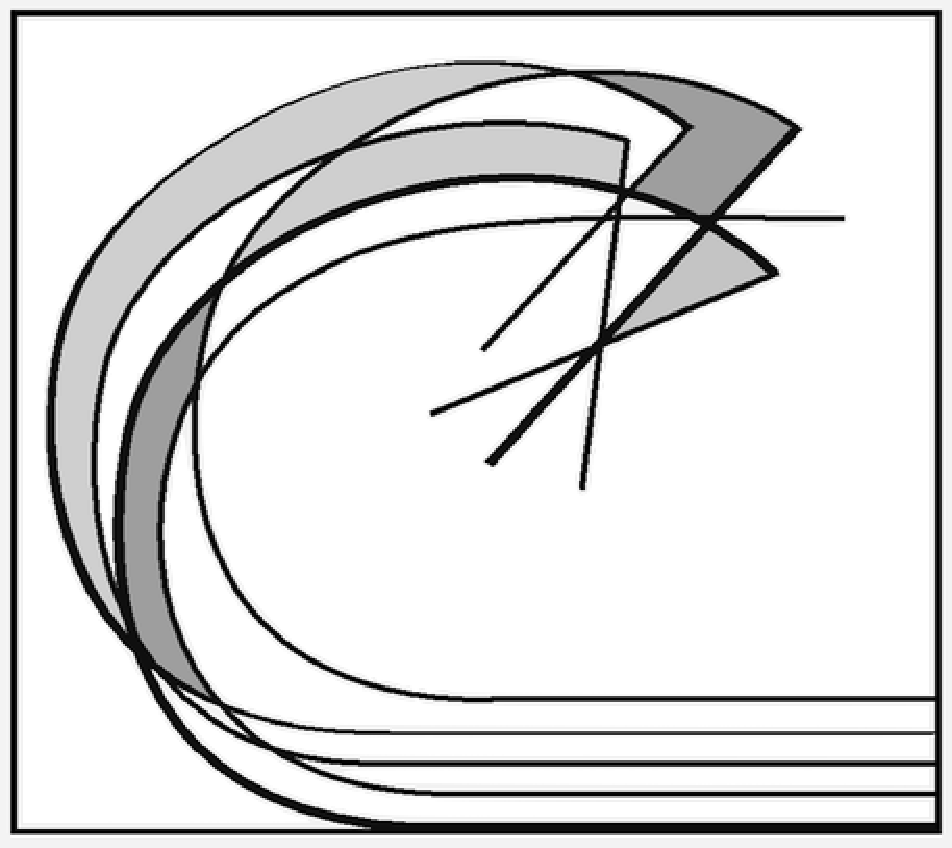
\includegraphics[scale=0.172]{Conservatorio.pdf}} & \LARGE \spacedlowsmallcaps{Conservatorio di Musica}\\ 
& \LARGE \spacedlowsmallcaps{S. Cecilia di Roma} \\ \cmidrule{2-2}
& \spacedlowsmallcaps{DIPARTIMENTO DI} \\
& \spacedlowsmallcaps{NUOVE TECNOLOGIE E LINGUAGGI MUSICALI} \\
& \spacedlowsmallcaps{SCUOLA DI MUSICA ELETTRONICA} \\
\end{tabular}
\end{center}
\label{default}
\end{table}%   

%        \LARGE \spacedlowsmallcaps{Conservatorio di Musica S. Cecilia di Roma}
%        
%        \bigskip
%        
%        \hrule
%        
%        \bigskip
%        
%        \large \spacedlowsmallcaps{DIPARTIMENTO DI NUOVE TECNOLOGIE E LINGUAGGI MUSICALI}
%        
%        \spacedlowsmallcaps{SCUOLA DI MUSICA ELETTRONICA}
        
		\vfill
        
        \spacedlowsmallcaps{CORSO DI DIPLOMA ACCADEMICO DI SECONDO LIVELLO IN}
                       
        \LARGE \spacedlowsmallcaps{MUSICA ELETTRONICA}

        \vfill 
        
        \begin{figure}[htbp]
\begin{center}
\includegraphics[width=.75\textwidth]{Insinuarsi.pdf}
\end{center}
\end{figure}

        \LARGE {\color{Maroon}\spacedallcaps{\myTitle}}
        
        \large \mySubTitle 
        
        \vfill
        
        \normalsize Candidato:\\
        \Large \spacedlowsmallcaps{\myName}
        
        \normalsize Matricola: \\
        \Large \spacedlowsmallcaps{4128BN}
        
        \bigskip
        
        \normalsize Relatore: \\
        \Large \spacedlowsmallcaps{Michelangelo Lupone}

     \normalsize Correlatori: \\
        \Large \spacedlowsmallcaps{Marco Giordano, Luigi Pizzaleo}



        \vfill ~ \vfill ~ \vfill
        
        \normalsize Anno Accademico: \\
        \Large \spacedlowsmallcaps{2018-2019}


%        \includegraphics[width=0.7\textwidth]{TFZSuperEllisse} \\ \bigskip
                   

    \end{center}        

\end{titlepage} 
 
\thispagestyle{empty}

\includepdf[offset=-80 0,
		    scale=1.43,
		    pagecommand={
		    	\begin{tikzpicture}[
					remember picture,
					overlay]
		    	\node [xshift=10cm,yshift=1cm] at (current page.south west) {\color{white}{
			Unamolla, \textit{particolare.} - Foto scattata durante la ripresa dei campioni di analisi, Roma. 2019}};
				\end{tikzpicture}}
		    ]{Unamolla_particolare_due.pdf}

\clearpage

\cleardoublepage

%!TEX TS-program = pdflatex
%!TEX encoding = UTF-8 Unicode

%*******************************************************
% Dedica
%*******************************************************
\chapter*{Dedica}

\pdfbookmark{Dedica}{Dedica}

Dedico: \\
\\
\textit{
a Federica, con la quale ho avuto quest'anno uno dei rapporti più profondi degli ultimi dieci anni \\
\\
a Togaci, con la quale condivido da sempre un percorso artistico e di ricerca \\
\\
a Danilo, che ha reso possibile l'esecuzione della mia composizione \\
\\
a Massimo, che ritorna sempre nella memoria per aiutare nei momenti più scuri e allietare nei momenti più chiari \\
\\
a Marco, che mi ha fatto compagnia nelle burrasche e nei mari limpidi \\
\\
a Daniele, Cristiano ed Alex, che in un modo o nell'altro, hanno intrapreso con me un viaggio che ancora non è finito e forse mai finirà \\
\\
ad Elena, piccola e sempre vicina figura che mi scruta da lontano \\
\\
a Cesarina, che ha tirato fuori dallo scrigno la mia identità \\
\\
a tutti, dedico, il mio insinuarmi nel vuoto
}

\pagestyle{scrheadings}

%!TEX TS-program = pdflatex
%!TEX encoding = UTF-8 Unicode
%!TEX root = ../2018-03-26-papa-vitres-de-son.tex

%*******************************************************
% Contents
%*******************************************************

\phantomsection
\pdfbookmark{\contentsname}{tableofcontents}
\setcounter{tocdepth}{2}
\tableofcontents
\markboth{\spacedlowsmallcaps{\contentsname}}{\spacedlowsmallcaps{\contentsname}} 

\cleardoublepage

\doublespacing

\pagenumbering{roman}

%!TEX TS-program = pdflatex
%!TEX encoding = UTF-8 Unicode
%!TEX root = ../2018-03-26-papa-vitres-de-son.tex

%*******************************************************
% Introduzione
%*******************************************************
\chapter*{Introduzione}

\pdfbookmark{Introduzione}{Introduzione}

\begin{flushright}
		\textit{Fatto sì è che qualsiasi creazioni mi ha sempre affascinato: vedere crescere le cose, essere create lì per lì sotto gli occhi... si tratti di una statua o di un quadro, o anche di un vestito nuovo, trovo che è sempre una nascita, una creazione che ha qualcosa di veramente emozionante. \footnote{Giacinto Scelsi, \textit{Il sogno 101}, Quodlibet S.r.l., Macerata 2010}}
	\end{flushright}

La musica elettronica è un mondo vasto, pieno di incantevoli afflati e meravigliose esplosioni. Un enorme calderone, ormai, di intenti, di sotterfugi e di bellezza, che tende a far trasparire a volte, i limiti dello strumento musicale o elettronico e allo stesso tempo le sue qualità. La tecnologia ci offre la possibilità di accedere a nuove tipologie di analisi e di elaborazione del segnale in tempo reale: questo deve essere un pregio del mondo contemporaneo, una spinta e non un riflesso. \\
Evitare la consequenzialità, la ridondanza, la ripetizione, è uno scopo che ho sempre cercato di raggiungere nelle mie composizioni. Riuscire ad avere una forma che mi desse la possibilità di far trasparire la continuità del tempo, come avviene al di fuori della composizione stessa e per quel postulato della fisica per il quale: 
\[ 
\textbf{"nulla si crea, nulla si distrugge, tutto si trasforma".}
\]
Continuamente il mio pensiero si dirige verso tale postulato. Considero la creazione musicale come un immagine mentale di un progetto, che rende possibile, nel reale poi, la trasformazione dei materiali grezzi in uno strumento: dall'informale al formale.
Lo strumento musicale nelle mani dell'esecutore o del performer, si tramuta in suono che dà vita alla composizione. Tale composizione indica un punto lontano da raggiungere che è la direzione musicale da noi scelta e non deve avere ambiguità esplicativa. \\ 
Questa tesi di ricerca è una sintesi di tali concetti: costruzione, analisi e composizione elettroacustica: formata da due movimenti, che prendono il nome di \textit{varchi}. I varchi temporali sono come i tempi che attraversiamo nella vita e, di seguito, ci lasciamo alle spalle, mantenendone la memoria. Ho tentato di insinuarmi in forme musicali strettamente connesse, all'interno di una timbrica rugosa ma nello stesso tempo lieve, alla maniera degli \textit{spettralisti}, dirigendo la mia attenzione ad un metodo legato ad attese di avvenimenti sempre differenti, ad affermazioni di gesti intensi, tramite un dialogo musicale che sfocia in un incastro così forte da diventare \textit{fusione}. \\
Spero che tutto ciò avvenga, in questi due varchi, che fanno il movimento dell'opera: \textbf{Insinuarsi nel vuoto}. 

\begin{small}
\begin{quotation}
\textit{Di ogni fenomeno si può fare esperienza in due modi. \\
Questi due modi non sono arbitrari ma connessi ai fenomeni - \\
essi vengono derivati dalla natura dei fenomeni, da due proprietà degli stessi: \\
esterno - interno\footnote{Wassily Kandisky, \textit{Punto, linea, superficie}, Adelphi Edizioni, Roma, 1968}}
\end{quotation}
\end{small}

Dopo la mia tesi compositiva del triennio \textit{Vitres de son, come un rosone nel cuore di un tempio immenso}, ho portato avanti la mia ricerca sui \textit{mollofoni} e sullo studio dello spettro inarmonico e la sua capacità di interagire con materiali sonori legati a strumenti di liuteria classica, come il brano \textit{Trapassato dal Futuro}\footnote{Trapassato dal futuro, composizione per Violoncello, Sp.I.R.E. e \textit{live electronics}, 2018, Prima assoluta: Istitut Goethe, Roma} scritto nel 2018 per il CRM (Centro di Ricerche musicali) di Roma, nella manifestazione \textit{ArteScienza 2018}. \\
La possibilità di interazione tra strumenti come violoncello o strumenti a fiato come il sassofono soprano\footnote{Presente nei due movimenti composti per la tesi}, è un ambito di ricerca che mi è molto a cuore da anni e che cerco di analizzare, facendo mio il concetto in ogni composizione. \\
L'ambito di ricerca è inerente allo spettro inarmonico della molla e alla sua capacità di divenire familiare ai suoni dell'ambiente cittadino nel quale siamo immersi. Finalmente eliminare gli ideali, per rendere familiare la composizione colta ad un ambiente, a tratti ostico, dove la direzione musicale prende un altro percorso: essere presente nella vita quotidiana e rendere intellettualmente più interessante il mondo circostante, dargli una forma per scrostargli quella caratteristica ansiogena e macchinosa che vuole dargli il capitalismo. Non fuggire da un ambiente comune che ormai abbiamo creato, ma dargli uno spiraglio per l'ispirazione e farlo diventare fonte di creazione. \\
Infine, ho focalizzato la mia creazione dello strumento ad una delle parti: la molla. \\
Finalmente la molla viene amplificata da un microfono a contatto e due magneti che confluiscono in un'unica fonte sonora, prendendo il nome di \textbf{Unamolla}.

\pagenumbering{arabic}

% !TEX TS-program = pdflatex
% !TEX encoding = UTF-8 Unicode

%************************************************
\chapter{Inquadramento storico}
\label{chp:Inquadramento storico}
%************************************************

\section{La nuova musica}
Nella storia della musica fino ai primi del novecento, si è diretto l’interesse verso una realtà compositiva legata all’universo tonale e ad un’armonia ferrea e rigorosa, così per la forma, fissa su nomenclature e ripartizioni classiche. Con il passare degli anni e con l’avvio della \textit{scuola di Darmstadt}, si sono andate ad ideare nuove tecniche compositive e ad inventare nuove forme stilistiche. Come scrive Henri Pousseur nelle conclusioni del suo libro \textit{Musica, semantica, società}:
\begin{quotation}
\textit{“ [...] quando è necessario, tagliare i rami che impediscono lo sviluppo armonioso dell’insieme, azione violenta in modo esemplare (purché prudente)! \\ 
L’arte moderna potrà sviluppare fin d’ora i modelli di ciò che Marcuse chiamerebbe il “lavoro libidinoso” (anticipando in tal modo esigenze di un stato di pace ancora sconosciuto), soltanto se non trascura di denunciare nello stesso tempo, nella maniera più efficace possibile, ciò che ancora impedisce (con la feroce durezza che sappiamo) a questo stato di pace e a questa possibilità di gioiosa creazione collettiva di diffondersi su tutta la faccia della terra! In questa prospettiva penso che è perfettamente lecito dar ancora prova di un po’ d’impazienza, di invitare con urgenza agli indispensabili scossoni. Anzi, sarebbe imperdonabile restare senza far nulla! Lo si voglia o no, il tempo dei flauti e delle cornamuse, di cui occorre intuire e far intuire la felicità, è attualmente ancora imperdito da quello della tromba, del tamburo e del Grido.” \footnote{Henri Pousseur, \textit{Musica, semantica, società}, traduzione di Eugenio Costa per Casa editrice Valentino Bompiani \& C. S.p.a., Milano, 1972}}
\end{quotation}
Di questa citazione bisogna selezionare alcune parti fondamentali, ed eventualmente puntare la nostra lente d'ingrandimento su delle questioni assai più complesse. L'idea di stralcio, di taglio, può avvenire solo nel caso non si fanno i conti con la tradizione e si renda del tutto inutile il legame con il passato. Questo, però, non avviene, dato che, per quanto il serialismo sia una tecnica che rompe con la tradizione, rimane legato a molte forme e a molti universi compositivi interni alla cultura classica: si cambiano le metodologie "armoniche", ma si rimane ferrei all'interno di schemi ben definiti. \\
\MakeUppercase{è} con la nascita di una figura importantissima per la musica contemporanea che si inizia a delineare un nuovo scenario legato al\textit{la nuova musica}: il \textbf{tecnico audio}. Lo studio di fonologia di Milano, lo studio di GRM di Parigi, Lo studio elettronico di Mosca, nella figura dell'ingegnere Eugenij Murzin, la nascita di molte radio legate agli studi di ricerca sul suono, sono i baluardi di questo immaginario sonoro nel quale oltre la musica scritta a livello notazionale si iniziano a scrivere algoritmi e schemi legati ai sistemi di diffusione. Il suono non è più delimitato all'interno di altezze legate al mondo temperato. Già con Ligeti, Hàba e Wyschnegradsky si concentrarono in Europa numerose esperienze teoriche, sperimentali e compositive che prevedevano l’uso di \textit{microintervalli}, grazie anche all'utilizzo del calcolatore, che rendeva possibile accostamenti ritmico-melodici difficili da concepire a livello classico (ad esempio l'accostamento di un vasto numero di oscillatori che differivano di pochi herz l'uno dall'altro o la nascita della modulazione di frequenza).\\
Lo stesso Bruno Maderna sostenne, durante un concerto presso Darmastadt del 1959, in riferimento ad una sua composizione, \textit{Musica su due dimensioni} (1952):

\begin{quotation}
[...] ho imparato che la musica è un'arte del tempo, perché fino al momento dell'esecuzione si deve dar forma e ordinare l'imprevedibile e perché io come compositore mi trovavo di fronte a me stesso come interprete. Nell'ambito della musica strumentale queste due funzioni sono state sempre più separate: io scrivo una partitura e la dò all'interprete, [...] la responsabilità della realizzazione sonora è nelle mani di un'altra persona dotata di proprie idee, e capacità. Una sintesi di entrambe le possibilità esistenti che io chiamo "dimensioni" mi sembra particolarmente fruttuosa, dal momento che l'interprete, nell'incontro con le realizzazioni sonore fissate sul nastro, fatte dallo stesso compositore o da lui controllate, raggiunge un contatto molto pi
 stretto con l'autore. [...] Io ho avvertito per la prima volta nel 1952 la necessità di questa sintesi, e ne fui felice, poiché ho sempre desiderato di collegare la composizione e l'interpretazione\footnote{Francesco Galante Nicola Sani, \textit{Musica Espansa, Percorsi elettroacustici di fine millennio}, Casa Ricordi LIM Ediitrice, 2000}.
\end{quotation}

Per Luigi Nono "la musica deve saper intervenire nella situazione contemporanea, nella storia contemporanea"\footnote{\textit{ibidem}} e così accade, anche grazie alla nascita di \textit{regie del suono} e figure come Alvise Vidolin, Antonio Farina, Nicola Bernardini e molti altri, prendono forma e rendono possibile pensare ad una composizione, oltre che nella sua natura di scrittura, anche come messa in scena. Così con il tempo si innesca un nuovo approccio alla musica e al suono che prese il nome di \textit{musica elettroacustica}.

\begin{quotation}
Nello studio elettronico si possono trovare direttamente diverse possibilità di concretizzazione di strutture sonore, che attraverso manipolazioni di concretizzazione di strutture sonore, che attraverso manipolazioni continue si possono rinnovare e mutare all'infinito [...], e come il tempo ora si presenti come un campo vastissimo di possibilità. Noi ora proviamo propensione a questo tipo di pensiero, non più lineare e di condotta presente anche nella musica strumentale [...]\footnote{\textit{ibidem}.}
\end{quotation}

Può apparire anche quasi antico il discorso che continuo a sottolineare in questo capitolo, dato che sembrano ormai ben saldi questi paradigmi e quasi alla base della musica elettroacustica che ogni giorno andiamo ad analizzare. Rimane però questo piccolo particolare, l'emozione per una cura al dettaglio, una cura alla necessità di esprimere un concetto, tramite un metodo. Sottolineo questo concetto, perché è proprio la cura al particolare, ma anche ad una calma interna, che dà la possibilità di soffermarsi su caratteri musicali e compositivi per me estremamente necessari come il timbro e le micro-variazioni tonali.

%************************************************************************************

\section{Il legame con il passato}

\subsection{Spettralismo}
Ad oggi, la business music ha rivelato migliaia di generi musicali legati alla musica elettroacustica ed elettronica ed è riuscita a catalogare in moltissimi insiemi e sottoinsiemi il mondo musicale. In passato, però, più che di genere musicale, si parlava di corrente artistica, prima che le etichette discografiche diventassero delle vere e proprie \textit{direzioni artistiche} e prima che si imponessero le leggi di mercato, si parlava appunto di correnti e in questo capitolo mi vorrei soffermare su una di esse: lo  \textit{spettralismo}. \\
Se con la nascita dello \textit{spettralismo} abbiamo la crescita di una musica composta per strumento ma resa più ricca timbricamente anche grazie all’ausilio dei computer, grazie all’analisi spettrale e alla possibilità di creare maglie di suoni fino a quel momento sconosciute, in seguito con la musica elettroacustica si ha la possibilità di unire questi due mondi creando un’ambiguità sonora notevole. \\
Nella maggior parte dei casi si andava a ricercare la modifica a livello di altezze e in qualche modo anche di "amplificare" le capacità timbriche di uno strumento tramite l’utilizzo di campionamenti differenti dei file di ripresa eseguiti in precedenza o tramite vari filtraggi, ricordiamo il brano per sassofono e nastro magnetico di Jean-Claude Risset: \textit{Voilements}. \\
Lo sviluppo di nuove tecnologie e di tempi di elaborazione del suono sempre più puntuali, ha reso possibile l'elaborazione del suono dal vivo e la possibilità di rendere sempre più complesse le creazioni degli \textit{algoritmi} presenti anche in partitura che venivano ideati dai compositori, come Luigi Nono, Luciano Berio, Michelangelo Lupone e moltri altri maestri della musica contemporanea che hanno utilizzato, nel connubio tra tecnica e arte, queste \textit{invenzioni compositive e tecnologiche}. \\
Proprio sulla base dello studio compositivo e tecnologico che mi vorrei soffermare. Ovviamente se uno strumento musicale viene utilizzato solo nelle sue tecniche classiche, il divario tra elettronica e strumento classico sarà difficile da colmare. Quindi, già nell’utilizzo della \textit{spazializzazione} che nell’elaborazione dal vivo, questo divario è diventato sempre più piccolo. Luciano Berio con i suoi studi sugli strumenti e in seguito Giorgio Netti e molti altri, tramite la scrittura e l’utilizzo di tecniche estese sempre più precise e complesse, sono arrivati al vivo dell’argomento. La risposta finalmente non è fuori, nell’utilizzo di un’elettronica troppo più potente degli strumenti canonici, ma è dentro, nella ricerca di tecniche estese che possano portare lo strumento ad essere vissuto in tutta la sua pienezza timbrica, frequenziale e di ampiezza sonora. 

\subsection{La ripresa microfonica}

Lo studio delle tecniche estese e la possibilità di cogliere qualunque sfumatura di uno strumento viaggia a pari passo con l’evoluzione della tecnologia. Finalmente microfoni creati \textit{ad hoc} per riprendere determinate qualità di uno strumento e una miriade di effetti di ambiente\footnote{riverberi a convoluzione, ad esempio}, diventano quasi un prolungamento dello strumento di liuteria classica. Questo non per sminuire l’interesse verso uno strumento musicale del quale possiamo apprezzare anche acusticamente le sue qualità, ma molto più per accentuare le qualità timbriche: una \textit{lente di ingrandimento sul suono}. C'è un importanza della ripresa microfonica anche a livello compositivo: il microfono in una nuova modalità deve diventare fido compagno del compositore, il quale, dovrebbe iniziare ad apprezzare ogni strumento non solo nella sua natura acustica ma anche nel suo \textit{essere amplificato}. In un’idea ormai antica ma mai rimarcata: \\
\[\textbf{strumento musicale + microfonazione}\] \\
Fausto Romitelli, compositore rimasto in attività fino al 2004, esigeva la microfonazione dei suoni strumentisti e non disdegnava l'utilizzo di uno svariato numero di diffusori. In \textit{Professor Bad Trip, Lesson I} possiamo vedere come una soluzione ritmico-melodica è scritta per far assaporare un fittizio \textit{eco} da parte degli archi tramite una ripetizione e una diminuzione graduale del volume indotto negli attacchi: 
\begin{figure}[htbp]

\begin{center}

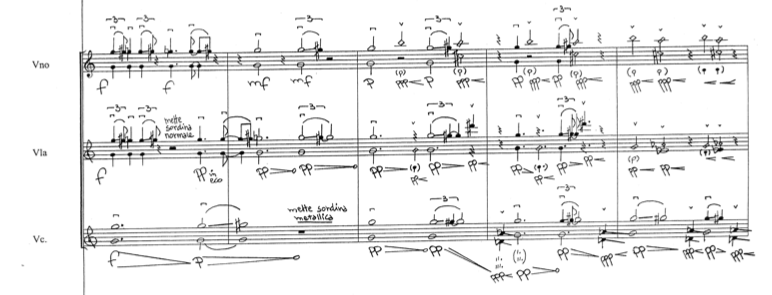
\includegraphics[width=1.\textwidth]{Romitelli_01.png}

\caption{particolare partitura \textit{Professor Bad Trip, Lesson I}}

\label{fig:01_Romitelli}

\end{center}

\end{figure}

La presenza del microfono diventa, come detto, una vera e propria lente di ingrandimento sul suono, che ci fa apprezzare e trasformare in arte compositiva e quindi in gesto, anche le micro-variazioni frequenziali e di ampiezza e di spettro che lo strumentista va ad eseguire. Ciò ha portato a partiture più accurate e con questo ad una maggiore attenzione da parte dello strumentista a cogliere fino alle più piccole sfumature legate allo strumento.

\begin{quotation}
Una netta contrapposizione - in suoni di combinazione - tra stabilità (suono normale) e instabilità (suono raschiato) porta a inaspettate e sorprendenti relazioni certamente da considerare - tra le altre - come primarie\footnote{Simone Santi Gubini, \textit{Difettosità timbrica e subarmoniche}, Masterclass Emufest  2017, Roma}.
\end{quotation}

\subsection{L'elettronica}

La parte riservata all’elettronica in questo caso diviene un ulteriore supporto, se non proprio un ulteriore indagine verso nuove idee compositive. Non c’è più bisogno di ricercare negli intervalli armonici o inamornici dei cavilli per uscire o rientrare in un panorama moderno, si può lavorare in micro-mondi atonali che si muovono anche all’interno di una o due note\footnote{N.B.: in questo caso parlo di nota non per indicare l'universo temperato, ma solo per semplicità: lavorare su altezze molto vicine, che poi siano note precise come un do, o che sia un do monesis calante o un fa, poco importa. Il fine è il raggiungimento di una nostra soluzione compositiva, con la quale, partitura dopo partitura, riusciamo a redigere un corollario di gesti e notazioni che, se spiegate, si possono eseguire di nuovo alla stessa maniera. \\}. Ovviamente, i grandi maestri come Nono ci indicano il cammino e rendono possibile avere una traiettoria, una base, dalla quale poter partire:

\begin{quotation}
Per esempio si prenda un suono, Si\textit{b.} Oggi è possibile con la tecnologia, con il \textit{live electronics} (o senza) utilizzare una parte del suono, una parte dell'aria o, improvvisamente, tutto il suono, con una direzione particolare e un'intensità particolare, fino a terminare solamente con un soffio. Allora non c'è più un Sib, ma il flautista viene a utilizzare il soffio più vicino al Si\textit{b}, e il \textit{live electronics} permette di esaltarlo. Tutto questo è ciò che con la tecnica si può ottenere oggi da un solo suono che eravamo abituati a considerare molto preciso, uniforme, unitario. [...]  è impossibile riconoscere il cambiamento di un clarinetto contrabbasso a una tuba a sei pistoni, o a un mezzosoprano, quando suonano estremamente piano. Non è possibile per il motivo che tutti gli strumenti, tutte le sovrapposizioni degli elementi armonici del suono, scompaiono\footnote{Luigi Nono, \textit{La nostalgia del futuro, Scritti scelti 1948-1986}, Gruppo editoriale Il Saggiatore s.p.a., Milano 2007}.
\end{quotation}

La notazione rediviva si colora di metodo, sempre più incalzante, sempre più denso di nozioni che servono a far intendere ciò che il compositore vuole e dove vuole arrivare, la piena coscienza del suono e delle modalità di esecuzione per arrivare a tali corrispondenze. \\
\textit{Insinuarsi nel vuoto} è il nome con il quale ho marchiato questo \textit{dittico}, un viaggio in due mondi, paralleli e lontani, ma limitrofi e adiacenti, nei quali provo ad unire suoni lontani, quasi atavici, in complesse (almeno per me) forme musicali. Nei capitoli successivi andrò a sviscerare la comparazione tra strumenti classici e \textit{Unamolla}, così da rendere più coscienzioso e intimo il contatto con la parte compositiva, perché solo penetrando e passando al microscopio alcune parti della materia, si può cogliere a pieno il suono che, tramite la diffusione, si disperde nell'aria. Concludo con una citazione da \textit{On Sonic Art} di Trevor Whishart, che si riferisce a questo campo e riguarda uno strumento ancestrale, quanto contemporaneo: la voce.

\begin{quotation}
[...] musical gesture is evidenced in the internal morphology of sound-objects and also in the overall shaping of groups, phrases, etc. [...] the morphology of intellectual-physiological gestures [...] may be translated directly into the morphology of sound objects by the action of the larynx, or the musuclature and an instrumental transducer. The translation of performance-gesture into the gestural-structure of the sound-object is most complete and convincing where the technology of instrument construction does not present a barrier\footnote{Trevor Wishart, \textit{On Sonic Art, a new and revised edition edited by Simon Emmerson}, Published in The Netherlands by Harwood Academic Publishers, Amsterdam, 1996}.
\end{quotation}







% !TEX TS-program = pdflatex
% !TEX encoding = UTF-8 Unicode

%************************************************
\chapter{Strumento di nuova concezione}
\label{Strumento di nuova concezione}
%************************************************

Come non cadere nel fascino della creazione tramite "tavole musicali" come avviene
in Cage o evitare di intraprendere un percorso musicale legato al teatro, dove
diventa più importante il gesto stesso che la composizione e la forma? Semplice,
tramite un'analisi specifica degli strumenti in questione.

Appena la nostra ricerca, da ammaliante, diventa analitica, allora il tutto
diventa più chiaro e si perdono anche le facili sperimentazioni sulla realtà e
si va a conoscere una bibliografia sempre più estesa e ci si perde, verso, appunto,
l'ignoto.

Reputo essenziale nella vita di un compositore di musica elettroacustica,
l'avvicinamento al mondo \textit{liuteristico} e di costruzione, semplicemente
perché il realizzare qualcosa di fisico, comporta il contatto con la materia e
la possibilità di avvicinarsi \textit{con mano} al suono che si vuole andare a
formare, o modificare e trasformare.

La scuola del compositore che immagina, scrive, e solo in seguito dà vita alle
proprie opere, a mio parere, è ormai lontana, perché sovviene un nuovo
importante aspetto legato al suono: la complessità spettrale legata alle
armoniche, alla fusione e l’evoluzione di formanti, ma soprattutto alla caduta
di un regime tonale e di armonia classica, verso \textit{micro-variazioni} e
\textit{micro-ritmiche} legate sia all’universo microscopico che a quello macroscopico.

La fisica è giunta ormai a studiare delle parti sempre più piccole della materia,
poiché proprio all’interno del più piccolo frammento di essa si può trovare la
nostra origine e delle risposte legate all’evoluzione.



%************************************************


\section{Unamolla}

Indico \textbf{Unamolla} come \textit{strumento di nuova concezione}, uno
strumento composto da "una molla" in ferro armonico, una base in legno e un
sistema di amplificazione a contatto.

% Paolo Zavagna, in alcuni suoi appunti pubblicati sul suo sito
% internet\footnote{http://www.zavagna.it/paolo/}, redige una classificazione
% degli \textit{strumenti musicali elettronici}, qui definisce gli strumenti
% \textbf{Elettromagnetici}:

Facendo riferimento alla classificazione indicata da
Zavagna\footnote{http://www.zavagna.it/paolo/}, % il link deve puntare all'articolo preciso
degli \textit{strumenti musicali elettronici}, egli così definisce gli strumenti
\textbf{Elettromagnetici}:

\begin{quotation}
Gli strumenti musicali elettromeccanici che producono il suono tramite un’azione
meccanica di riproduzione di una forma d’onda, che può essere "scritta" su un
nastro in movimento o su un disco rotante.
\end{quotation}

Unamolla è quindi, uno strumento elettromagnetico di nuova concezione.

\subsection{Passaggio da installazione a strumento}

Nel 2018, quando ideai \emph{Sp.I.R.E.} [installazione di molle e piastre regolate ed
elettrificate], notai subito che un difetto assai visibile era la trasportabilità.

Se in passato bastava scrivere una partitura e nell’eventualità trasportare il
mio personal computer, ora avevo creato un “oggetto” costruito appositamente per
tale scopo e (per quanto ci fosse un progetto alle spalle) molto cose erano
riproduzioni fisiche di schizzi creati con carta e penna. In seguito, tramite le
mie ricerche sulla performance musicale e lo sviluppo di varie tecniche per la
gestualità sullo \emph{Sp.I.R.E.}, decisi di utilizzare un oggetto sonoro per volta,
dedicandomi ad un limitato numero di parti: due. Utilizzai quindi \textit{Unamolla}
in acciaio ed una piastra in rame\footnote{le prime erano in ferro armonico e
zincato, le seconde in acciaio}; infine, decisi di dedicarmi ad un unica parte
e limitai la mia attenzione esclusivamente alla molla.

Se \emph{Sp.I.R.E.} era uno strumento composto da 4 molle e 2 piastre in grado, tramite
degli attuatori, di auto-eccitarsi, Unamolla è uno strumento meno complesso nella
costruzione, ma più complesso nel sistema di ripresa. Lo \emph{Sp.I.R.E.} aveva come
sistema di ripresa solo 4 microfoni a contatto e due microfoni posizionati ai
lati per donare una stereofonia all'ascolto. Nel caso di Unamolla, invece, la
diffusione è \textbf{mono} ed è più complessa dello \emph{Sp.I.R.E.}, perché è in realtà
una somma di più fonti di ripresa sonora collocate sullo strumento.

\begin{figure}[t]
\centering
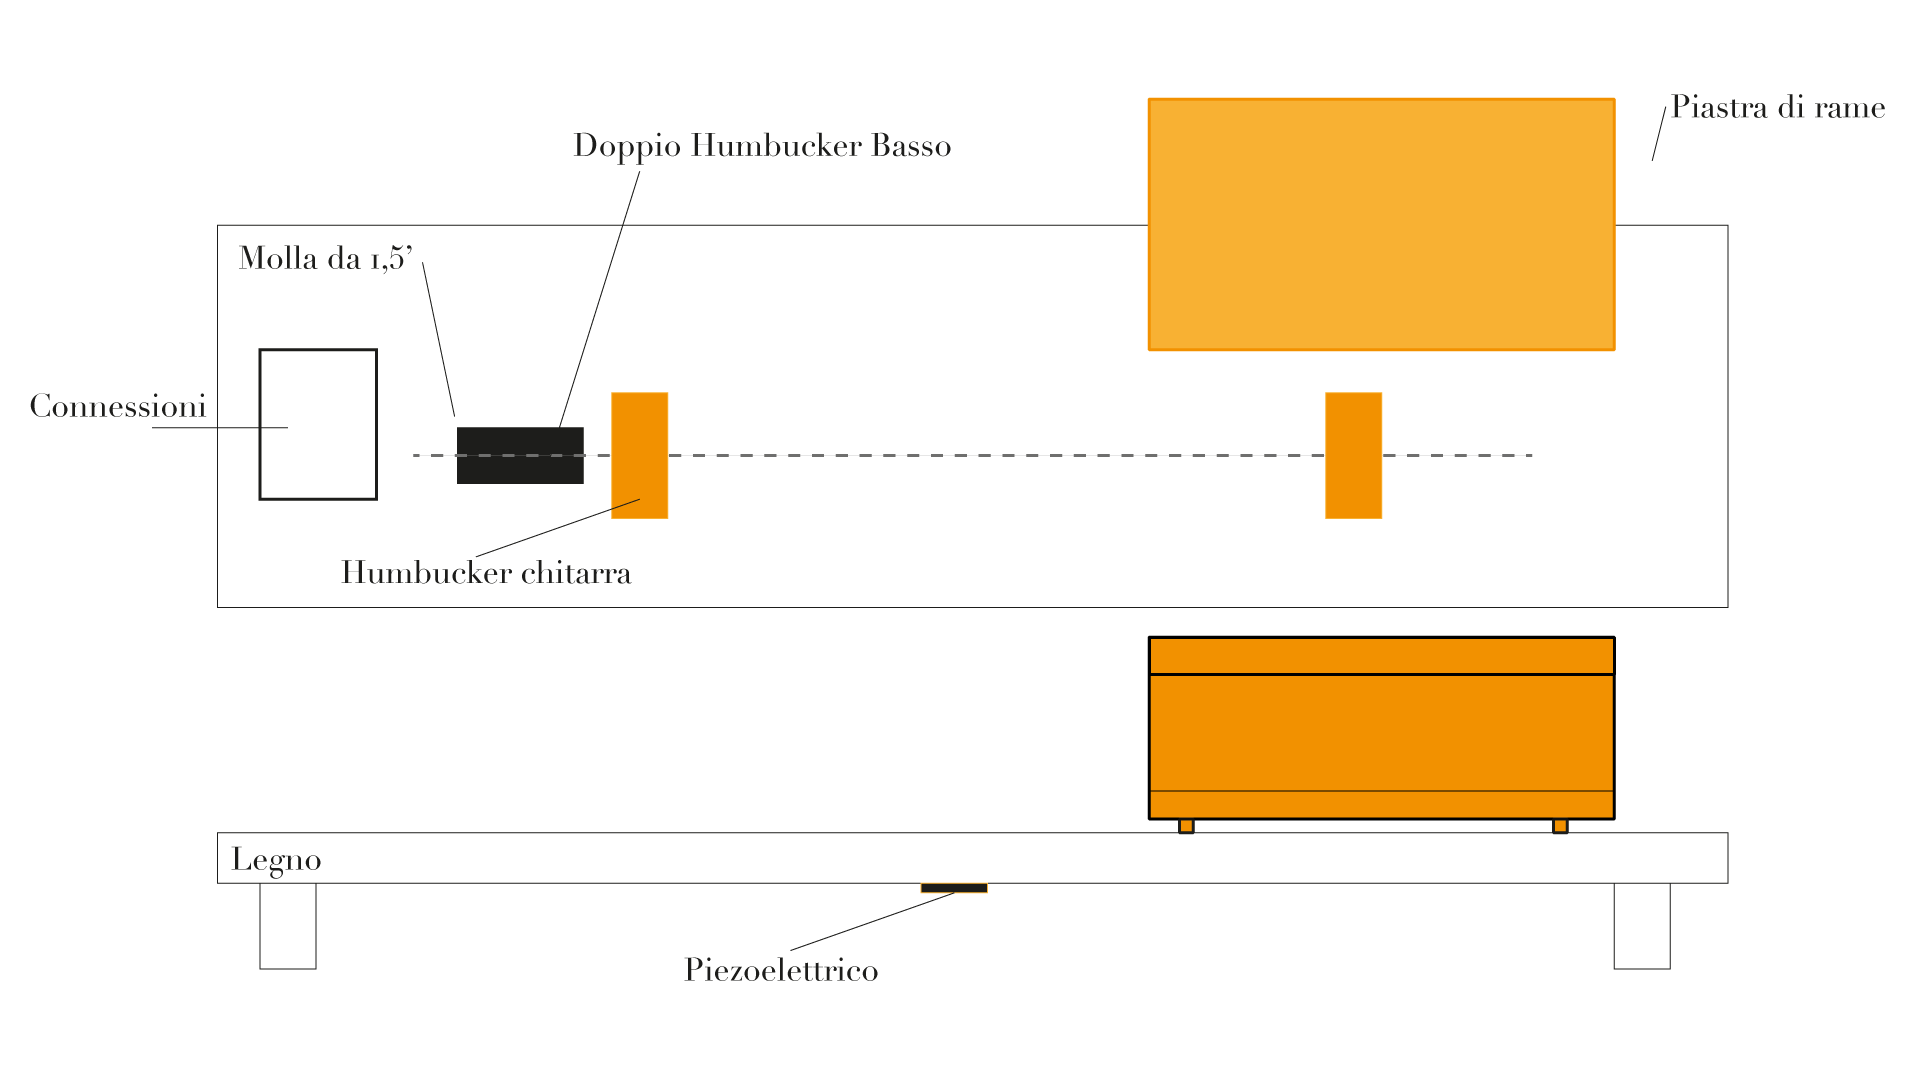
\includegraphics[width=1.\textwidth]{unamolla_schema.png}
\caption{Schema \emph{Unamolla 1.0}}
\label{fig:02_unamolla_01}
\end{figure}

\subsection{Sistema di amplificazione \textit{UNAMOLLA}}

Durante la costruzione dello \emph{Sp.I.R.E.}, avevo notato che il segnale non era
trasdotto perfettamente (utilizzavo solo dei piezoelettrici), mancava di attacco
e le dinamiche erano davvero piatte. Aggiunsi quindi su una tavola di legno,
prima uno, poi due humbucker (per chitarra e per basso) in aggiunta al
iezoelettrico e fui soddisfatto del risultato. Ho potuto, quindi, definire
\textit{Unamolla} come \textit{strumento musicale} ed iniziare la mia analisi
gestuale.

Unamolla si può definire uno strumento a \textbf{spettro inarmonico} costituito,
nel primo prototipo, da una lastra di ottone e di una molla in ferro-armonico,
connesse da una tavola di legno di noce. Questo primo prototipo, che ho chiamato:
\emph{Unamolla 1.0}, ha subìto con il tempo delle variazioni ulteriori dalla figura che
segue e, con il tempo ho diminuito ulteriormente la sua grandezza e ho diviso
piastra e molla.

In figura \ref{fig:02_unamolla_01}, lo schema di costruzione di \emph{Unamolla 1.0}.

Nello schema è disegnata la tavola di legno sulla quale è fissata una molla da
1,5 pollici e la piastra di rame, opportunamente disaccoppiata tramite una vite
inferiore al contatto con il legno e una vite superiore di fissaggio. Sul lato
sinistro della molla ho posto un doppio Humbucker per basso elettrico ed in
seguito, ho diviso, alle due estremità, i due humbucker per chitarra. Al di
sotto della parte in legno troviamo un piezoelettrico.

\emph{Unamolla 1.0} è stato il primo stadio, il primo prototipo di strumento. Anche se
le dimensioni erano estremamente diminuite, la trasportabilità dello strumento
era ancora in fase di cambiamento, dato che ogni volta dovevo smontarlo e
montarlo, ma soprattutto alcuni gesti erano difficilmente eseguibili.

Decisi quindi di lavorare su una seconda \textit{Unamolla}  e ho creato il secondo
prototipo: ho eliminato la lastra (come scritto in precedenza) per dare spazio
ad un design più consono per eseguire determinati gesti legati anche all’uso
dell’archetto.

%************************************************
\section{Analisi acustica}

\begin{figure}[t]
\centering
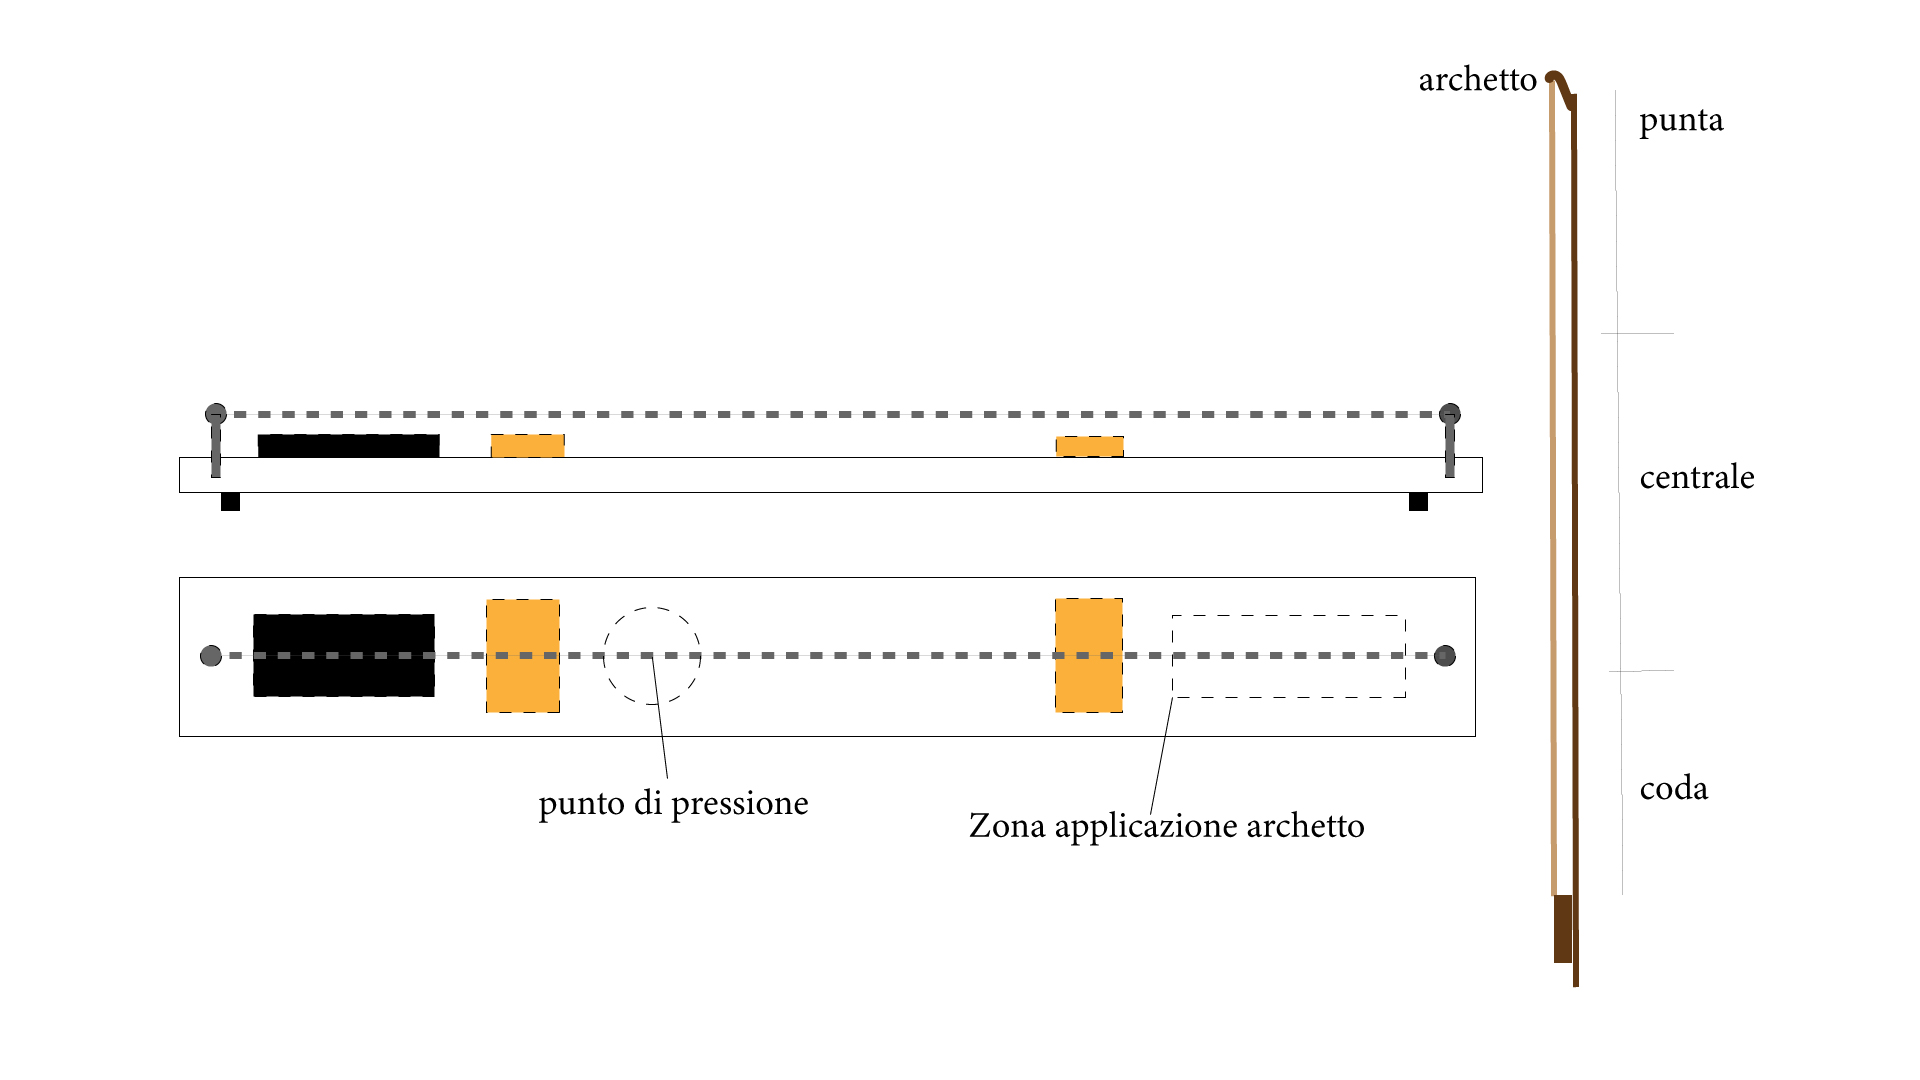
\includegraphics[width=1.\textwidth]{unamolla_schema.jpg}
\caption{Schema Unamolla 1.2}
\label{fig:03_unamolla_02}
\end{figure}

L’analisi acustica di uno strumento amplificato di nuova concezione come
\emph{Unamolla} ha molteplici gradi di variabilità legati soprattutto alla
gestualità dell’esecutore ed alla molteplicità di modalità eccitative della molla.

Non disponendo di una prassi esecutiva consolidata, è importante codificare in
modo preciso e, quanto più possibile, riproducibile, i parametri che determinano
il gesto e la modalità di eccitazione dello strumento.

Per iniziare un approccio di analisi ad Unamolla, ho deciso di utilizzare un
archetto barocco per violoncello e restringere il range di analisi a determinati
gesti.

Come si nota in figura 3, ci possiamo avvalere di vari parametri per l’analisi
di un'arcata, applicata direttamente sulla parte tratteggiata a destra.

\subsection{Tecniche di ripresa}

Tutte le riprese sono state fatte con una scheda audio e sono a $48KHz$ e $32bit$.

I campioni sono tutti mono e il segnale che otteniamo è la risultante della somma
(tramite saldatura) di:

\Large{\color{red} COME TI HO SCRITTO NELLA NOTA PRECEDENTE, TRAMITE SALDATURA NON SIGNIFICA NULLA SE C'è UNA SOMMA è TRAMITE SOMMA ANALOGICA DIRETTA, SENZA INTERVENTI DI AMPLIFICAZIONE O RIDUZIONE DEL GUADAGNO}

\begin{itemize}
  \item{Doppio Humbucker per basso}
  \item{Doppio Humbucker per chitarra}
  \item{Piezoelettrico}
\end{itemize}
\Large{\color{red} dovresti indicare le specifiche tecniche di quello che hai usato, se trovi diagrammi, nomi, codici. È una ricetta con ingredienti scelti.}

\Large{\color{red} separa la parte acustica da quella gestuale e musicale}

Di seguito diamo le definizioni dei parametri gestuali presi in considerazione
con i relativi range di valore:

\begin{description}
  \item[Archetto:] come mostrato in figura, consideriamo le tre zone punta, centrale, coda.
  \item[Angolazione archetto:] l’angolazione presa in esame è quella nell'ambito $30\sim70^\circ$.
  \item[Velocità:] lento, veloce, moderato.
  \item[Tensione:] molla libera oppure fermata con la sola pressione di uno o due dita della mano libera.
  \item[Pressione:] da 0 a 10, considerando lo zero con l’archetto semplicemente appoggiato, e il 10 come uno \textit{sf}.
\end{description}

Prendiamo in esame, un determinato gesto che ha queste caratteristiche:
\begin{description}
  \item[Zona dell’archetto:] coda
  \item[Angolatura:] $60^\circ$
  \item[Velocità:] lento
  \item[Tensione:] molla fermata che tocca la base in legno a 1/3 a destra.
  \item[Pressione:] 2
\end{description}

\Large{\color{red}Ho cambiato lo spettro, ovviamente non so se fa riferimento allo stesso campione}

In figura \ref{fig:04_spettro_01}, lo spettro in frequenza del gesto.

\begin{figure}[h]
\centering
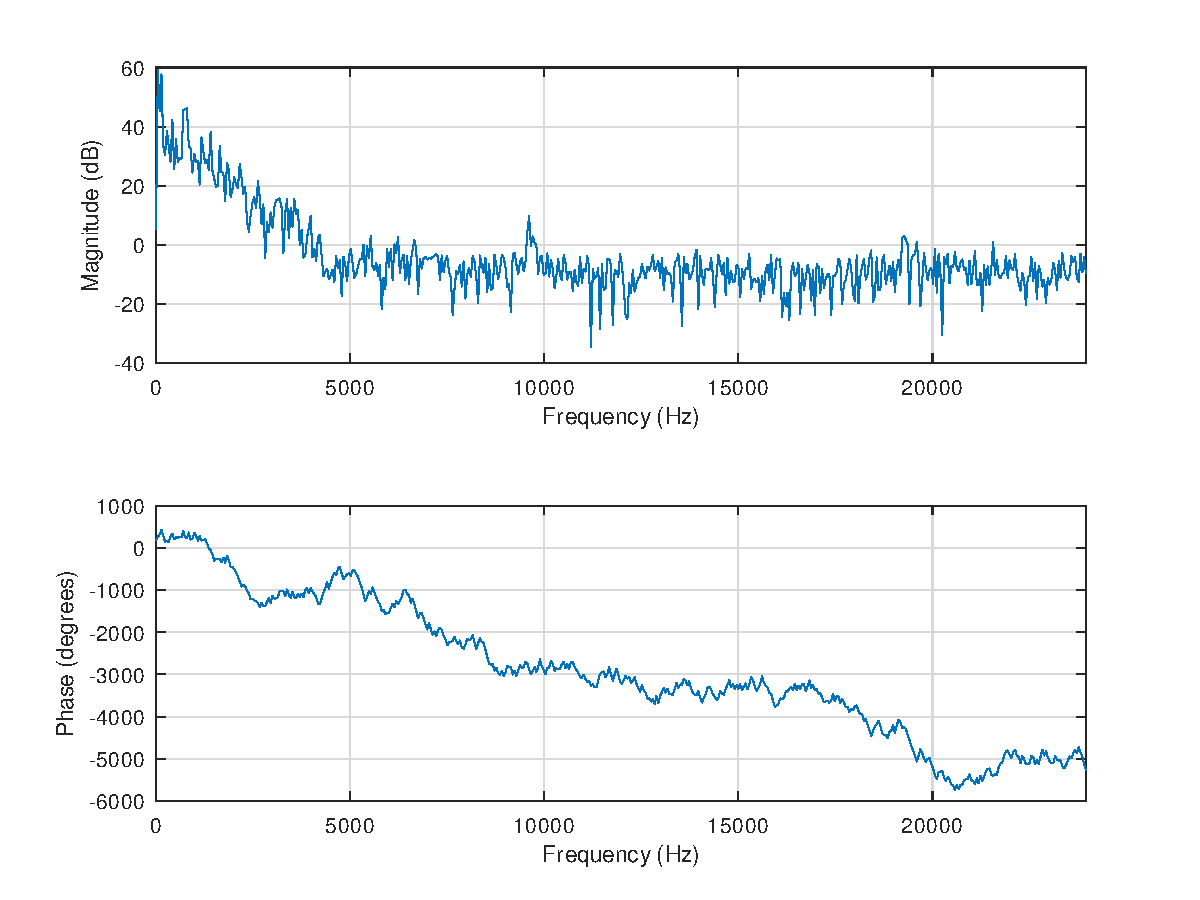
\includegraphics[width=1.\textwidth]{unamolla_octave}
\caption{Unamolla, analisi spettro}
\label{fig:04_spettro_01}
\end{figure}

Nell’esecuzione di ogni gesto emergono degli aspetti legati all’interazione
dell’esecutore con lo strumento e al feedback tattile alimentato dalla reazione
dello strumento stesso all’intervento dell’esecutore. In questo caso la reazione
più evidente è che tutto l’avambraccio e la mano avvertono una tenue modulazione
sulle basse frequenze dovuta alla vibrazione della molla sulla base di legno.
Questa vibrazione rimane fino ad una velocità moderata, con una pressione a
0.4-0.3 (in una scala da 0 a 1) e rimane fissa per tutte le zone dell’archetto,
ma va a perdersi quando la pressione e la velocità aumentano, dato che entra in
gioco un nuovo fattore che è legato sia alla vocalità dell’archetto, sia della
molla: la molla inizia a vibrare di meno sulle basse frequenze e lo strofinio
dell’arco si intensifica fino a suonare da sé.

La bassa frequenza cerchiata è quella che crea quella rugosità del suono che
possiamo apprezzare soprattutto a molla ferma con il dito e nella zona dell’archetto
vicino alla coda verso il centro. Inoltre, all’interno dello spettro sottostante
si possono identificare le punte degli inviluppi formantici. Uno a $130Hz$ e l’altro
a $750Hz$. Durante l’esecuzione di questa parte, ho notato una vocalità ben precisa
dello strumento, a circa 130 hertz (appunto) che come vediamo nello spettro
successivo, si identifica in una parziale di una curva formantica. Facendo dei
conti,

\Large{\color{red} che conti? riporta i tuoi calcoli.}

ho notato che se si considerano determinati bin che compongono la curva
formantica, si può notare come il MCD è intorno a $10\sim18Hz$, nella figura notiamo
un movimento non in banda audio a circa $18Hz$. La parte nel cerchio rosso è sui
$36Hz$, la prima delle parziali che compongono uno spettro che di base è inarmonico,
ma tramite determinati accorgimenti si può accentuare tale sua vocalità e rendere
possibile la costruzione di determinati gesti ai fini del nostro volere compositivo.
Riuscire anche a muoverci (o forse solamente a muoverci) in un universo micro-tonale.

Un altro fattore molto importante, notato durante l’esecuzione del gesto, è l’alta
variabilità di suono che avviene anche con il cambio dell’angolatura dell’arco:
a $45^\circ$ e $60^\circ$ i crini dell’archetto non si incastrano con le spire della molla.
Ovviamente può essere compositivamente interessante anche sfregare i crini
all’interno delle spire della molla, ma in quel caso abbiamo bisogno di un
archetto con poca pece, perché in quel caso la pece renderebbe difficile il
movimento dell’archetto facendo incastrare le spire con le sezioni di crini che
si vanno a formare.

Quando muoviamo l’archetto sulla molla, ci scontriamo con la pressione, che va
dosata, dato che ogni parte dell’archetto per via della tensione, suona in modo
differente, quindi a seconda della frizione e della velocità, va mosso l’archetto
in modo adeguato per creare un suono che risulti continuativo, che per gli scopi
compositivi personali è molto importante.

Venendo da una composizione come L’albe nei varchi, che precede il solo con la
molla in questo trittico, ho decisamente bisogno di un suono che sia in fase
iniziale continuativo e soggetto a micromovimenti che possano rendere il movimento
continuo non ripetitivo e che abbia realmente una direzione compositiva adeguata
al mio stile.

\textbf{Come si nota dalla seguente analisi di spettro-frequenza, dell’attacco
dell’archetto sullo strumento, ci sono due curve formantiche intorno a $100Hz$ e
a $700Hz$.}

\subsection{Considerazioni sull’amplificazione}

Ho preferito limitare il campo di ripresa agli elettromagneti e ai microfoni a
contatto, perché sono inerenti all’elaborazione del Live Electronics che andrò
ad effettuare e soprattutto sono gli unici tre canali che amplifico. Ho deciso
di unire tutte le riprese audio in un’unica uscita fisica.

Non ho notato cancellazioni fisiche del segnale. L’unione delle fonti sonore
è il risultato di varie prove effettuate per avere più dinamica ma soprattutto
più presenza dello strumento e uno spettro più ricco. La somma dei segnali è
poi il reale suono che ho ricercato per la molla.

In futuro, come esplico nello schema in figura 5, cercherò di creare una cassa
di risonanza \textbf{a lunghezza variabile} con la quale poter enfatizzare e
modificare l’amplificazione del mio strumento e non delimitare più il campo di
amplificazione al contatto, ma estenderlo ad una microfonazione differente
(tramite la cassa di risonanza ed un microfono a condensatore).

\begin{figure}[h]
\centering
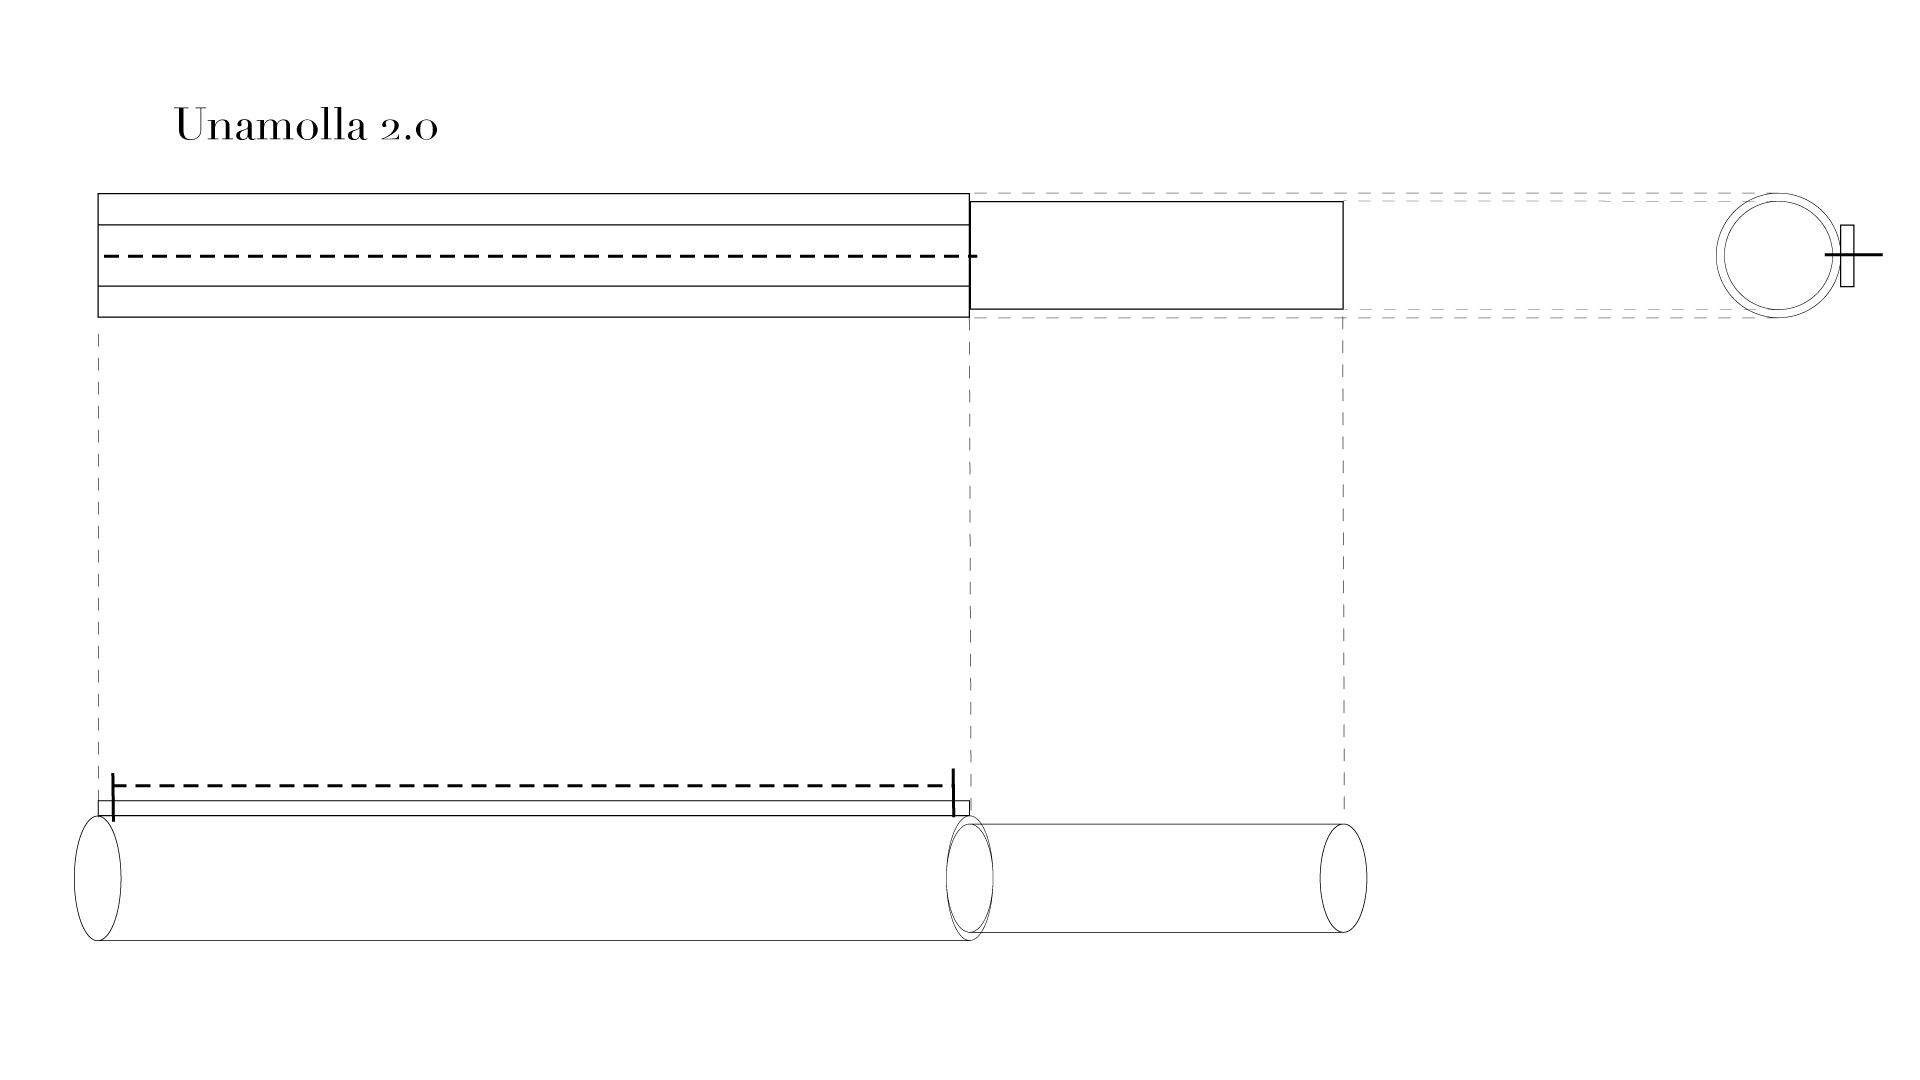
\includegraphics[width=1.\textwidth]{unamolla_2_schema.png}
\caption{Unamolla 2.0, design di Unamolla con cassa di risonanza variabile}
\label{fig:05_unamolla_2.0}
\end{figure}

\subsection{Conclusioni}

Le prime domande che mi sono poste era riguardo la comparazione con strumenti
reali e la possibilità di farli convivere all’interno di una partitura.

Per quanto riguarda lo \emph{Sp.I.R.E.} ho intrapreso uno studio gestuale molto legato
al mondo percussivo. Nel caso di Unamolla, ho deciso di avvicinarmi più al mondo
degli archi e l’analisi gestuale inizia con l’utilizzo di un archetto barocco
per violoncello. I parametri in gioco sono diversi, l’idea di trovare una
vocalità nello strumento sta appunto nella convivenza di vari fattori.

L’archetto è stato posizionato al margine sinistro della molla. La molla è stata
“fermata” con un dito creando una sorta di nodo a 1/3  dal margine destro, subito
dopo il primo humbucker per chitarra da destra. Abbiamo tre parametri che entrano
in gioco, in base ai quali è stata fatta la classificazione del gesto sono i
seguenti, legate a determinati parti della molla sulla quale avviene la speculazione.

\begin{description}
  \item[Velocità:] dato che parliamo di uno strumento pluri-amplificato,
    si nota subito, al tocco, che tra lento e moderato può rientrare un universo di
    micro velocità che scaturiscono interessanti spunti di ricerca.
		\item[Tensione:] molla libera, fermata con la sola pressione di uno o due dita
		della mano libera dell’archetto. Questa seconda tipologia di tensione ha come
		risultato l’eliminazione delle \textit{auto-vibrazioni} indotte alla molla e
		la possibilità quasi di “intonarla”. Inoltre si può fermare la molla anche
		facendole toccare la base in legno sempre pigiando con un dito nella parte
		centrale; il risultato sarà una frequenza più alta della precedente e pari
		quasi al doppio della frequenza precedente: $130Hz$. Questo comporta un indice
		di vibrazione sulle basse frequenze della molla, che diminuisce (o addirittura
		quasi scompare) quando viene fermata.
		\item[Zona dell’archetto:] Come per la velocità, queste parti contengono un
		mondo di microgesti che se uniti anche a velocità e modifiche della tensione,
		riescono a trasformare minimamente il suono inarmonico, riuscendo (anche
		tramite un’elaborazione) a eccitare la molla a tal punto da riuscire a
		sottolineare una vocalità intrinseca dello strumento.
		\item[Pressione:] ultimo ma non meno importante parametro, rende possibile
		il cambio timbrico della molla ed entrano in gioco parti inerenti all’archetto
		stesso e ad armoniche che possono venir fuori nel momento in cui si uniscono
		vari fattori, tra cui una determinata posizione dell’archetto, la velocità e
		la pressione. Ho adottato una scala da 0 a 1, dove 0.01 ad esempio è
		l’archetto in movimento semplicemente poggiato, e 1 è uno sf. Bisogna avere
		molta cura nella pressione dell’arco, perché al minimo sbaglio suona l’arco
		stesso, quasi a parere un armonico, e dirige l’attenzione dell’ascoltatore
		verso frequenze molto acute, tralasciando le medio basse che perdono di
		intensità.
\end{description}

\textbf{Tutti questi fattori possono essere riportati in partitura per precisare
a quale suono si vuole puntare tramite un determinato gesto.}

\textit{Nella difficoltà esecutiva di uno strumento con uno spettro complesso
come quello della molla, possiamo sentire risuonare vari strumenti, come trombe,
corde di contrabbasso e anche una minima vocalità se si vanno ad enfatizzare
delle parti specifiche dello spettro.}



%************************************************

\section{Catalogazione degli strumenti, gesto-segno}

Per avvicinare al mondo degli strumenti musicali di liuteria classica, lo strumento
Unamolla, ho deciso di intervallare la performance-solo dello strumento, con due
composizioni: una per sassofono soprano tape ed elaborazione; un duo per
strumento e sassofono tenore. Prima di iniziare la scrittura del duo, ho deciso
di stabilire dei parametri sui quali lavorare, delle parti simili a livello
spettrale tra i due strumenti. In primo luogo ho pensato ai multifonici e in
seguito, nella parte del duo, alla quantità di rumore indotta nello strumento
tramite un soffio più deciso nell'insufflazione  con cambiamenti della posizione
del labbro inferiore.

La catalogazione che segue, è stata ideata per riuscire ad individuare gesti
simili tra questi due strumenti di famiglie differenti: una appartenente all’universo
temperato, l’altra, al contrario, appartenente all’universo della molla, in teoria
più vicina a quello dei rumori.

Insieme ad un violista abbiamo riscontrato che ci sono varie parziali all’interno
dello spettro della molla, come si può riscontrare anche nell’analisi. C’è una
nota principale che è il LA, ma attorno, nello spettro della molla si possono
definire sia un Si che un Sol diesis crescente che un La un’ottava superiore e
un Sib.

Esistono varie aree di studio con le quali possiamo lavorare per avere un approccio
reale all’unione di strumenti occidentali e strumenti di nuova creazione:

\begin{description}
  \item[gestuale:] come detto in precedenza, studio legato al gesto fisico e
	successivamente alla creazione di un segno o simbolo che, ben spiegato in
	legenda, rende possibile l’esecuzione di una determinata cellula musicale;
  \item[comparativa:] strumenti reali in comparazione agli strumenti di nuova
	creazione;
  \item[compositivo:] unione ritmico-melodica su base formale e timbrica.
\end{description}

A livello umanistico si stanno facendo ad oggi delle indagini riguardo il gesto.
Non più una visione solo temporale dell’utilizzo di varie tecniche, ma anche
spettrale e spaziale. Lo strumento d’analisi è, quindi, nel dominio congiunto
di tempo e frequenza. Ovvero, tramite software specifici si dà spazio ad
un’analisi che ha come base lo studio delle armoniche o delle accentuazioni a
livello frequenziale in determinati gesti fatti sullo strumento.

\subsection{Strumenti a confronto: catalogazione}

Per fare un’analisi completa delle tecniche ho voluto stilare una serie di
tecniche e gesti uguali per ogni strumento che vado ad analizzare. E’ ovvio che
l’utilizzo delle chiavi è strettamente legato al flauto, ma a mio parere
documentare tutte le tecniche rende ancora più palese la possibilità di rendere
omogeneo questo studio.

\begin{table}[htp]
\caption{Sassofono Soprano, tabella comparativa tecniche}
\begin{center}
\begin{tabular}{ccc}
\hline
\textbf{Tecniche/Strumento} & \textbf{Unamolla} & \textbf{Sassofono Soprano} \\
\hline
Pizzicato & SI & NO \\
\hline
Grattato & SI & NO \\
\hline
Flautato & SI & SI \\
		&con archetto & \\
\hline
Nota lunga & SI & SI \\
		&con motore & \\
\hline
Nota corta & Mallet & SI \\
		&in metallo & \\
\hline
Trillo & NO & SI \\
\hline
Frullato & SI & SI \\
		&con motore & \\
\hline
Glissato & NO & SI \\
		& & ma solo su \\
				& & piccoli intervalli \\
\hline
Vibrato & NO & SI \\
\hline
Variazione & SI & SI \\
di quarto di tono & con motore & \\
& o archetto & \\
\hline
Variazione di tono & SI & SI \\
& solo se si crea & \\
& un nodo centrale & \\
\hline
Fruscìo & SI & SI \\
\hline
Soffio & NO & NO \\
\hline
Chiavi & NO & SI \\
\hline
Armonici & SI & SI \\
\hline
Bicordi & NO & MULTIFONICI \\
\hline
Tricordi & NO & MULTIFONICI \\
\hline
Accordi & NO &NO \\
\hline
\end{tabular}
\end{center}
\label{default}
\end{table}%

Come possiamo vedere dalla prima tabella, alcune tecniche che sono di natura come
per uno strumento come il SASSOFONO SOPRANO, diventano un po’ più complessi da
riprodurre per la molla. Ad esempio il frullato non può essere riprodotto, ma
può venire eseguito dalla molla tramite un motorino continuo (vibratore o rasoio
per capelli). Ho voluto anche specificare la presenza o meno dell’archetto con
la molla per poter scrivere più precisamente anche i segni inerenti alla natura
della tecnica eseguita sul nuovo strumento. Ultimo gesti presente in Unamolla è
legato al suo feedback. Tramite un overdrive della BOSS e un CRY-BABY (pedale wah-wah)
ho la possibilità di eccitare determinate armoniche della molla e di riuscire,
tramite il pedale, a controllare il feedback, riuscendo a definire dei piccoli
cambiamenti microtonali.


% !TEX TS-program = pdflatex
% !TEX encoding = UTF-8 Unicode

%************************************************
\chapter{Lo studio compositivo, tratti e indicazioni gestuali}
\label{chp:Lo studio compositivo, tratti e indicazioni gestuali}
%************************************************

\epigraph{Passa l'infinito di lì, passa la luce, non c'è bisogno di dipingere [...] invece tutti hanno pensato che io volessi distruggere: ma non è vero io ho costruito, non ho distrutto. \\ Lucio Fontana, \textit{Concetto Spaziale - Attese, 1961}}

Pensare di costruire un suono e al contempo distruggere tutto il passato solo grazie ad uno stralcio con la cultura precedente, penso sia un passo al quanto azzardato, nonché inutile. Il contatto con il passato non è soltanto un punto di passaggio nel quale fare tappa, ma diventa un cardine, un punto di slancio, con il quale argomentare qualunque percorso presente proiettato nel futuro che si va a ideare. \\
La notazione, se si parla di strumenti entrati ormai da centinaia di anni nella tradizione, dovrà essere pressoché classica e piena di quei piccoli accorgimenti che possano far interagire in maniera piena l'esecutore con lo strumento.

\section{Dal paragone all’indipendenza del suono}

Dopo aver effettuato le mie analisi di comparazione tra spettri armonici e inarmonici e aver individuato delle somiglianze e delle differenze all’interno dei due, ho anche notato nei miei studi di musicologia che alla base di molte ricerche musicali abbiamo soprattutto quest’idea di “comparazione” tra strumenti di liuteria classica e parti elettroniche o oggetti sonori a spettro inarmonico. Di base però l’idea di comparazione allontana, a mio parere, dal vero senso di interazione tra gli strumenti che dovrebbero essere semplicemente l’inizio di una ricerca personale sul suono. Non è più la ricerca di sembrare o apparire un suono quanto un altro, ma semplicemente lavorare su una proprio immagine spaziale e sonora. \\
L’interazione tra gli elementi dovrebbe essere un mezzo e non il fine del nostro lavoro compositivo. L’unione dei due è solo un ennesimo algoritmo che ci da la possibilità di creare e comporre la nostra musica. Quindi, non più una ricerca che vada ad investigare verso un \textit{merge} tra i segnali, o utilizzare una modulazione ad anello per avere una modulazione tale da poterla integrare nel metodo, ma avere un’idea ben chiara sul proprio processo compositivo che è l’unione di tutti questi mezzi verso un’idea compositiva attuabile e intellegibile, ben salda. \\
Mi riferisco alla possibilità di fare una musica dove sia intellegibile il pensiero compositivo, se questa possieda o no rugosità o un’armonia interna. \\
L’idea di utilizzare la microfonazione come una lente di ingrandimento sul suono, che viene catturato 

\section{La stesura della partitura}

In questi anni di conservatorio ho lavorato molto sulla stesura di partiture sempre più complesse ma che potessero allo stesso tempo essere di facile comprensione. Facili nel senso in cui ogni simbolo rappresentasse un gesto ben definito e se ci fossero più gesti sovrapposti, o un gesto che rendesse possibile più suoni, annotarli tramite specifici simboli. 
Ho quindi creato un corollario\footnote{vedi \textit{cap. 2}} come abbiamo prima osservato nel caso della molla, dove ogni rigo o parte di esso, rappresenta una parte del gesto e che siano semplici da intendere nella loro complessità di sovrapposizione. \\
Per quanto riguarda la notazione, cerco sempre di trovare dei trattati, come avviene per il primo dei miei due movimenti, dove ho inserito un numero finito di figure scritte nel \textit{II trattato Netti/Weiss}. Questa composizione vuole essere una ricerca tra tecniche estese dello strumento e connubio con un’elettronica alla base semplice sia a livello frequenziale che di algoritmica, proprio per unire una complessità esecutiva con una semplicità nell’elettronica che però rafforzi e ravvivi l’intenzione sullo strumento e la sua preponderante forza espressiva. Nella partitura, come si può notare nella figura a fine paragrafo, ci sono i multifonici per lo strumentista e al di sotto di questi, i vari campioni, collocati nel punto in cui sono collocati nel missato.
\begin{figure}

\begin{center}

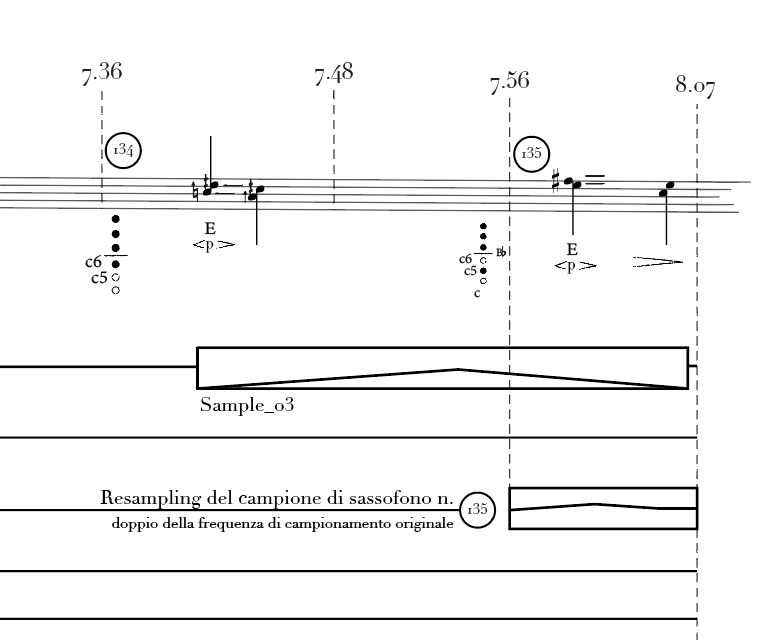
\includegraphics[width=1.\textwidth]{Partitura_particolare_01.jpeg}

\caption{Partitura: particolare}

\label{fig:01_Partitura_particolare_01}

\end{center}

\end{figure}


%************************************************

\subsection{L'utilizzo di una nuova notazione partituriale}

Come per lo \textbf{Sp.I.R.E.} (\textit{Spring installation Regulated and Electrify}), anche per Unamolla ho utilizzato uno nuova notazione e nuovi gesti, legati alla fisica dello strumento, ma senza allontanarmi troppo dall'eseguibilità del pezzo e l'eventuale riproduzione in futuro, da parte di chi, Unamolla, non la possiede, ma la può ricreare tramite lo schema e suonare, leggendo la partitura, da sé.

\begin{quotation}
Since music began to be notated, clearer distinctions between the work and its performance, and between the composer and performer, have emerged, representing multifarious views of the role of the performer.\footnote{Tanja Orning \textit{Pression} (a performance study) Norwegian Academy of MusicMusic Performance Research Copyright © 2012 Royal Northern College of Music Vol. 5}
\end{quotation}

La ricerca di nuove tipologie di notazione sta alla base della prassi strumentali, ovvero tecniche estese e tecniche compositive, ma anche nella creazione di una simbologia per l'elettronica, che risulti identificativa e allo stesso tempo espressiva. \\
Nella stesura del \textit{nastro magnetico} e nell'elaborazione ho preferito fare un catalogo dei miei campioni e dell'elaborazione di questi in modalità differenti, per il primo movimento e di elaborazione in tempo reale tramite filtri ed equalizzazioni in guadagno sullo strumento \textbf{Unamolla} per il secondo.

%************************************************

\section{Elaborazione del suono}

L'elaborazione del suono, dove aver preso in considerazione l'inquadramento storico e la capacità della ripresa microfonica come lente d'ingrandimento sul suono, diventa un vero e proprio prolungamento dell'esecuzione dello strumentista. Quindi, come accennato nell'introduzione, si ricerca un sentiero dove fondere l'elettronica e la parte eseguita su strumento. Ovviamente l'elaborazione ha necessità di esistere solo ed esclusivamente se viene utilizzata esclusivamente per scopi compositivi. I fini compositivi sono quindi la base del nostro lavoro e se ci troviamo a lavorare per una commissione, come avviene per \textit{L'albe nei varchi, come fuggir del susseguir d'incanti}, il primo dei tre varchi che compone il mio lavoro di tesi, ci dobbiamo scontrare con vari fattori. \\
In primo luogo sia l'elaborazione che l'eventuale "nastro magnetico\footnote{\textit{Nastro magnetico} va ad identificare una traccia audio sulla quale uno strumentista si trova a suonare. Identifico con nastro magnetico, semplicemente una traccia audio, solo per questioni storiche, non perché ci sia necessità reale di un nastro magnetico}" devono essere "trasportabili", ovvero devono essere reperibili eventualmente in una cartella presente in un \textit{cloud} nella rete, in comune con lo strumentista e con il registra, così da poter essere montata in fase preliminare e di esecuzione dal vivo senza la presenza fisica del compositore. \textit{L'albe nei varchi} rappresenta un brano su \textit{commissione}, il quale deve possedere, per essere eseguito con pochi intralci, queste caratteristiche:
\begin{itemize}
\item{\textit{Trasportabilità}: deve essere possibile trasporta la traccia audio su qualunque dispositivo e l'elaborazione avere diversi gradi: a seconda della tipologia di tecnico presente in regia, se non è presente il regista-compositore ci deve essere la possibilità di riprodurre la traccia su qualunque diffusione presente, anche, eventualmente, in mono.}
\item{\textit{Riproducibilità}: se si utilizzano software specifici, controllare che ogni parte del pacchetto che noi andiamo a creare sia di facile apertura in ogni personal computer, o addirittura, creare vari pacchetti per l'esecuzione, utilizzabili con programmi differenti. Uno schema algoritmico semplice e puntuale può essere la base per la ricostruzione in sede di sound-check e prove.}
\item{\textit{Eseguibilità}, ultima ma non inutile caratteristica, avere varie versioni, studiando prima i luoghi nei quali il brano verrà riprodotto, sarà decisivo.}
\end{itemize}


% !TEX TS-program = pdflatex
% !TEX encoding = UTF-8 Unicode

%************************************************
\chapter{La composizione: Insinuarsi nel vuoto}
\label{chp:La composizione: Insinuarsi nel vuoto}
%************************************************

\epigraph{[...] è sempre quel vuoto dell’intervallo complesso, che fa il volume ulteriore, un vuoto che collega non un vuoto che separa. \\
Giorgio Netti, Masterclass EmuFest IX, 2016 \textit{Conservatorio Santa Cecilia}, Roma}


\textit{Insinuarsi nel vuoto} è una composizione che si divide in due parti, nominate varchi, e rappresenta in qualche modo il mio percorso compositivo degli ultimi anni. Il primo, \textit{L'albe nei varchi} appunto, è un brano per sassofono soprano, tape ed elaborazione tramite riverberi; il secondo è \textit{Insinuarsi, mosso contrario}, un solo per Unamolla e \textit{live electronics} che sfocia in un duo con il sassofono tenore: Unamolla, sassofoni e live electronics racchiudono un processo di studi fatto su strumenti musicali di liuteria classica e strumenti di nuova creazione.
\\ \\
I varchi, non vanno immaginati di fronte, come se si dovesse attraversarli, ma ai lati. Come nel caso di Bologna o di Torino, dove le arcate sono laterali. Ogni passo è un ascolto, ogni passo verso il centro è sempre piú incalzante, finché, non ci si rende conto che la via è lunga e il tutto si bagna di una luce nuova. 
La luca nuova, E2. rappresenta una planimetria intrinseca dello strumento. Si va ad indagare nel lontano passato di suono, per il momento sconosciuti. Non ci sono più artefatti, è il suono che prende forma, è il tempo che si dilata: il vuoto non è più intrinseco ma diventa formale, il vuoto è lo spazio nel quale il suono si disperde e questo vuoto, risuona. Diventa risuonatore incostante di un precipitare che si tramuta in tempo-frequenza tempo-timbro e tempo-dinamica. L’incostante sempre uguale senso della vita che crea la normalità. Dove da una parte c’è chi riesce a viversi questa discesa senza pensare e chi è in ascolto, sente la continua vibrazione dell’aria che colpisce il corpo nella caduta. Insinuarsi nel vuoto è questa caduta che non trova mai il suolo, ma nell’aprire gli occhi trova il buio e una continua brezza sulla pelle che fa il vivere e non il sopravvivere.
E mi dirigo verso il nuovo, verso lo sconosciuto e nel vuoto dello spazio che sta tra le spire si incastrano i crini dell’arco nella ricerca di una vocalità che resa all’interno della molla ed enfatizzata echeggia, si disperde. Come si disperde l’aria all’interno del sassofono, come il fiato si trasforma in suono che dalla cavità orale viene filtrato dall’ancia e della labbra per penetrare nel tubo, apparentemente vuoto. 

%************************************************

\section{Varco I: L'albe \textit{come fuggir nel susseguir d'incanti}}

È il primo quadro ideato per raccontare, tramite le composizioni e non nelle composizioni, un percorso musicale o, se si vuole, di vita, dove, attraverso l’utilizzo di tecniche compositive e quindi gestuali, si indica un cammino compositivo formale. La parte scritta per sassofono soprano è legata ad uno studio fatto sul Trattato II - Netti Weiss, dove utilizzo varie figure presenti nel libro che si legano ad una parte di elettronica ideata sull’elaborazione di parti vocali sul \textit{Sol} e \textit{Sib} dell'ottava del Do centrale.
I varchi, non vanno immaginati come attraversati, ma nelle parti laterali di un viale coperto. Come nel caso di Bologna o di Torino, cove le arcate sono laterali a questi tunnel. Ogni passo è un ascolto è una trasformazione, ogni passo verso il centro è sempre più incalzante, finché non ci si rende conto che la via è lunga e il tutto si bagna di una luce nuova. \\
La luce nuova è l'elaborazione nei riverberi, è la tecnica estesa, è il finale del brano, dove all'interno del tape entra un campione di sassofono, ricampionato ad una frequenza di campionamento più alta e questo rende possibile la dilatazione temporale del campione che tramite un fade-out muore nell'inizio della seconda parte.

\subsection{Attese, silenzio e spazi.}

Come sostiene Paolo Mauri, critico letterario e storico della letteratura, in \textit{Buio}:
\begin{quotation}
Buio e silenzio. Tra le due parole c’è un legame antico, anche se [...] non obbligatorio. Molti sono esploratori del silenzio che fatalmente incontrano anche il buio. Sul silenzio notturno riflette e scrive più volte Leopardi, che è un vigile guardiano della notte oltre che uno scrutatore appassionato del cielo stellato. Il silenzio notturno può portare orrore o quiete. Il sonno si coniuga anch’esso al buio e con il sonno il sogno, quest’altra misteriosa metà della vita umana che sfugge al nostro controllo e che forse, invece, ci controlla, liberando i nostri demoni interiori, le nostre anche e anche i nostri desideri. \\
Il buio tuttavia può essere anche riempito di rumori, di suoni, per esempio di musica. Allora noi entriamo consapevolmente nel buio alla ricerca di sensazioni e di emozioni. Le discoteche e anche i vecchi night quei luoghi, privi del suono e degli effetti speciali, perdono completamente di senso e di identità\footnote{Paolo Mauri, \textit{Buio}, Casa editrice Einaudi, Trento, aprile 2007}.
\end{quotation}
Il silenzio è stata una pratica musicale molto in auge negli anni ‘60. Fisicamente il silenzio non è possibile, perché se c’è movimento nei corpi (ad esempio respirazione) o movimento al di fuori (aria in movimento) creare il silenzio è praticamente impossibile. Si può però indurre un’ascoltatore a tale suggestione, se in precedenza troviamo un crescendo o semplicemente se prima c’è del suono e dopo viene a mancare. \\
Alcune pratiche di ascolto, come il giradischi o il lettore cassette o spesso il CD, sono legate ad un rumore di fondo fisso, dato da vari fattori fisici dello strumento stesso\footnote{il nastro ha un rumore di fondo alto, il giradischi ha comunque dei solchi e così via}, quindi, l’evoluzione nell’utilizzo all’interno della musica eseguita dal vivo in sistemi digitali, ha reso possibile passare da un sistema analogico, perciò infinito a un sistema digitale e finito. Il sistema digitale ha come lato positivo che è utilizzabile, con un’adeguata strumentazione, per indurre al “silenzio relativo”.
L’albe nei varchi è una composizione che gioca su questi interruttori, con i dovuti crescendo e diminuendo. \\
L'impossibilità di eseguibilità data dalle misure restrittive in auge in questo momento, mi hanno fatto decidere di operare diversamente. In seguito spiegherò le modalità con le quali ho concluso e realizzato il brano, fornendo alla commissione una versione \textit{studio} del mio brano. 

\subsection{Il rapporto con lo strumentista}

Il rapporto con lo strumentista è una fase fondamentale per la stesura del pezzo. Ogni strumento è differente dall'altro e anche la cassa toracica e le labbra di chi esegue il pezzo. Dico questo per osservare che a volte le posizioni presenti sui trattati\footnote{In questo caso il \textit{Netti-Weiss}} sono specifiche per l'esecutore che le ha eseguite e variano anche in modo minimo per un altro strumentista. \\
Il passaggio fatto è stato il seguente: stesura della partitura con le notazioni di Giorgio Netti ed in seguito invio del materiale al mio strumentista Danilo Perticaro. Danilo ha studiato la parte, redatto le giuste modifiche. Cambiata in seguito la partitura, ho inviato di nuovo il materiale a Danilo per l'accertamento delle correzioni.

\subsection{Il lavoro a distanza}

Importante ed essenziale è stata la presenza a distanza dello strumentista. Dopo aver chiesto al maestro Giorgio Netti di poter utilizzare le sue registrazioni\footnote{su internet sono presenti le registrazioni di ogni singolo multifonico presente nel trattato} per creare un missato tale da poter elaborare ed ideare l'elettronica, ho inviato il lavoro ultimato del tape e dell'elaborato stereo finale, per dare così a Perticaro la giusta suggestione e la precisa direzione musicale che volevo raggiungere. \\
Eseguite le parti, Danilo mi ha inviato un file nel quale era presente il suo sassofono e l'ho sostituito all'interno della mia workstation digitale. Ho proposto all'esecutore una registrazione continua e totale del pezzo, così da fargli assumere una continuità, con tutte le possibilità del caso: rumore di chiavi, respiri, intenzione. 

%************************************************

\section{Varco II: Insinuarsi nel vuoto, \textit{mosso contrario}}

\epigraph{
sólo agg. e avv. [lat. sōlus, e come avv. sōlum e poi sōlō]. – 1. agg. a. Di persona, che è senza compagnia di alcuno, che non ha nessun altro insieme o vicino: Solo e pensoso i più deserti campi Vo mesurando a passi tardi e lenti (Petrarca) [...] \\ \textit{dall'Enciclopedia online www.treccani.it}}


Se nel primo varco ho voluto fare interagire uno strumento di liuteria classica con un tape elettronico di elaborazione di un campione, nel secondo varco ho deciso di utilizzare Unamolla e solo nella parte finale avviene il connubio con il sassofono tenore. Unamolla\footnote{come abbiamo visto nel capitolo 2} è uno strumento, per il momento, inarmonico. Questo strumento viene elaborato e modificato nel suo corso di esecuzione, tramite 7 canali che \textit{splittano\footnote{ovvero, moltiplicano il canale mono in 7 canali differenti elaborati ognuno con un processo a sé stante}} il segnale, in 7 parti, per ricreare un eterno ritorno, ma nel ritorno c’è una modifica continua, proprio come indicava Nono con la sua nostalgia del futuro:

\begin{quotation}
[...]evoluzione e rivoluzione, due fasi strettamente conseguenti: mercé le cui forze propulsive, e specie quella anche violenta della seconda in cui violenza altro non è se non ampliamento della capacità umana, si attua la umana continuità. \\
la vita si realizza in forma talmente viva, ché il presente è già il passato nel futuro. \\
in modo analogo, ma da analizzare ogni volta concretamente nella diversità della sua concreta situazione, procede tra spazi tra suoni tra colori l'uomo-poeta\footnote{Luigi Nono, \textit{La nostalgia del futuro, Scritti scelti 1948-1986}, Gruppo editoriale Il Saggiatore s.p.a., Milano 2007}.
\end{quotation}

\subsection{La nostalgia del futuro}

Solo per Unamolla e live electronics, \textit{mosso contrario} è un brano per performer ideato sul modello di una serie di analisi avvenute in precedenza\footnote{vedi capitolo 2} e si legano tramite delle elaborazioni a una \textbf{FFT}\footnote{\textit{Fast Fourier Transform}} che servirà, nella fusione con degli specifici campioni di strumenti tradizionali a \textit{prolungare} o \textit{dilatare} il segnale.\\
Ognuno di essi viene inoltre elaborato, tramite una maglia di equalizzazioni in guadagno e appunto dei filtraggi. \\
Il performer esegue delle parti che \textit{ritornano} e allo stesso tempo sono in modifica nel tempo. \\
Per quanto riguarda l’estetica ho intinto a piene mano agli spettralisti e ad un'ambiguità timbrica che trasforma il timbro della molla in un timbro complesso e va verso una vocalità formatasi grazie alle varie equalizzazioni.


%************************************************

\section{Insinuarsi nel vuoto}

"Insinuarsi nel vuoto" non è un punto di arrivo, ma solo un inizio. Insinuarsi, vuol dire entrare in modo lento e con una certa premura, dovuta a fatti precedentemente successi, a poca visibilità (il buio, appunto). \\
L'insinuarsi è l'entrare all'interno di luoghi anche pericolosi, sofferti, è un immagine poetica che dirige la sua focalizzazione verso un universo, come la musica elettroacustica, che per quanto si conosca, rimane un universo pieno sempre di novità e contrappunti di intenzioni. \\
Dirigersi verso qualcosa di atavico, di ascoltato, di vissuto e di sempre inteso, ma mai riprodotto. Ora è tutto lì, come il \textit{Bagatto}\footnote{La seconda carta dei tarocchi, contrassegnata con il numero uno, che rappresenta l'artigiano, l'artista, l'iniziato, che intraprendere per la prima volta il suo viaggio}: sul tavolo della figura che rappresenta, ha tutti gli strumenti per cominciare, per rendersi ora conto della realtà delle cose e avere la capacità di seguire o meno il cammino.
\begin{figure}

\begin{center}


\includegraphics[width=.4\textwidth]{Il_bagatto.jpeg}

\caption{Bagatto, carta numero uno dei tarocchi}

\label{fig:il bagatto}

\end{center}

\end{figure}


% !TEX TS-program = pdflatex
% !TEX encoding = UTF-8 Unicode

%************************************************
\chapter{Algoritmica e diffusione}
\label{chp:Algoritmica e Diffusione}
%************************************************

\epigraph{<<Comporre vuol dire \textit{costruire} uno strumento>> \\ \textbf{Helmut Lachenmann}}

In quest'ultimo capitolo visioneremo le modalità di riproduzione dei due movimenti, ma soprattutto un fattore esplicato in precedenza molto importante per quanto riguarda la riproducibilità di una composizione: \textit{la trasportabilità}. Ogni composizione deve essere, a mio parere, soprattutto nel caso di commissioni, trasportabile da una piattaforma all'altra, da una DAW all'altra, ma soprattutto avere dei parametri da essere riproducibile anche senza il compositore presente. \\
Per quanto riguarda L'albe nei varchi, il metodo ideato è proprio questo: il brano è riproducibile anche mono e gli effetti che vengono aggiunto nell'elaborazione, ovvero i riverberi, possono essere utilizzati anche direttamente in un live elettronics \textit{in loco}.


\section{Legenda e algoritmica}

I due varchi hanno due algoritmi differenti. Nel primo abbiamo degli inviluppi segnati in partitura e tre riverberi differenti, così da avere tre dimensioni differenti per ogni parte: il tape, l'elaborazione del sassofono soprano e la modulazione ad anello.

\begin{figure}

\begin{center}


\includegraphics[width=1.\textwidth]{legenda_particolare_01.png}

\caption{particolare partitura \textit{Legenda, I Varco: L'albe}}

\label{fig:02_Algoritmo_01}

\end{center}

\end{figure}


\begin{figure}

\begin{center}

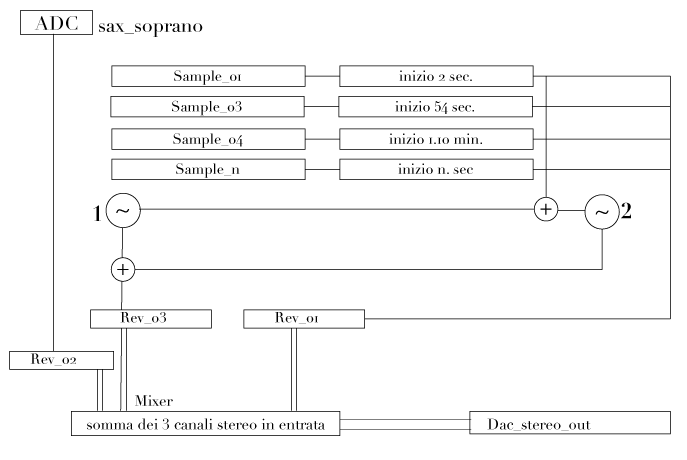
\includegraphics[width=1.\textwidth]{algoritmo_particolare_01.png}

\caption{particolare partitura \textit{Algoritmo I Varco: L'albe}}

\label{fig:02_Algoritmo_01}

\end{center}

\end{figure}


%************************************************

\section{Sistema di ripresa}

Il sistema di ripresa, date le condizioni di quarantena imposte dal decreto ministeriale dovuto al COVID-19, ho contattato il mio strumentista, Danilo Perticaro, e abbiamo optato per registrare in una piccola stanza con un microfono Zoom con ripresa stereo. I files mi sono stati inviati tutti a 44.1 kHz a 24bit. \\
Nel secondo varco, la ripresa microfonica, come esplicato nel capitolo 2, ho unito tre fonti sonore differenti presenti su Unamolla: 2 doppi humbucker e un piezoelettrico. Il tutto elaborato.

%************************************************

\section{Diffusione ambisonic} 

Le due composizioni, per quanto riguarda la riproduzione, erano state pensate per essere diffusione con più speaker. Purtroppo, data la situazione di emergenza non c'è stata la possibilità di farsi che questo avvenga e la soluzione è stata optare per due cambiamenti. Il brano \textit{L'albe} è diventato per diffusione stereo. In precedenza la mia idea era di utilizzare tre microfoni differenti e collocarli digitalmente, ognuno in una posizione diversa, modificando l'elevazione delle fonti, per dare una forma conica verso l'alto del suono del sassofono tenore. Tutta l'elettronica sarebbe stata collocata in tutti e 23 i diffusori della cupola e missata assieme al riverbero dedicato al sassofono che, come si può vedere in partitura, viene usato a livello compositivo, come gesto di continuazione dei multifonici del sassofono. \\
\textit{Insinuarsi nel vuoto, mosso contrario} invece, tramite decodifica \textit{binaurale} è stato trasformato per un ascolto in cuffia.  

\subsection{cupola di diffusori}
 
Entrambe le composizioni erano state ideate per essere riprodotte all'interno della cupola sonora presente nell'aula I, l'Aula Bianchini, al terzo piano del Conservatorio Santa Cecilia in Roma. Per via del cambiamento delle modalità di laurea, i brani sono rimasti entrambi in stereo. La decodifica ambisonic è stata sostituita da un ascolto frontale, stereofonico come si presenta negli algoritmi di costruzione. \\

% !TEX TS-program = pdflatex
% !TEX encoding = UTF-8 Unicode

%************************************************
\chapter{Riflessioni e conclusioni}
\label{chp:Riflessioni e conclusioni}
%************************************************

Le mie conclusioni? \\
Penso che ci troviamo, anche per via della società, ad inseguire nella vita, un immagine di noi stessi, tentiamo di cercarci al di fuori, quando la nostra essenza è semplicemente lì. Davanti lo specchio, nelle nostre esperienze di vita, ma soprattutto in un metodo. \\
Saper agire e non reagire, a mio parere, è il primo passo. \\
Ogni giorno, qualunque cosa accada, si rimane sempre un io “pulsante”. Non inteso come oggetto o soggetto, ma come corpo vibrante in connessione con tutte le energie umane e non, che ha attorno. \\
Non sto dirigendo le mie conclusioni, né il mio discorso, verso pratiche zen o olistiche; mi riferisco in modo assoluto alla semplicità con la quale sono arrivato, dopo tutti questi anni, ad intraprendere, ora, il mio cammino. 
\\ \\
Ogni algoritmo al suo interno ha un algoritmo più semplice, fino ad arrivare alle operazioni basilari, ogni scomposizione ritmica, anche di quelle più complesse, ha al suo interno una ritmica più semplice e così via. Così la nostra percezione del suono e della forma di esso può andare fino al midollo dello spettro e della percezione che abbiamo di esso. \\
A mio parere si dicono sempre pi\'u parole di quelle che servono e non si lascia quasi mai far respirare l'ambiente circostante, che avrà sempre al suo interno qualcosa da raccontare. \\
La semplicità che genera complessità, la possibilità di confrontarsi con un vuoto, una mancanza continua, che appena si percepisce, si annuncia e non preannuncia: si materializza. Da lì, abbiamo a mio parere solo due possibilità: la prima è colmarlo con espedienti, ideali, note. La seconda è provare a inseguire quel vuoto incolmabile che crea l’imprevisto, l’indagine, il seguire una ricerca e intraprendere un cammino nel buio, demarcato solo dai nostri intenti. Insinuarsi nel vuoto, infine, sempre con un briciolo di umiltà e uno sguardo verso il futuro, con quella nostalgia perpetua che non è freno, ma moto di un’estetica che non si trancia o si ricrea, ma si trasforma e modella costantemente come fa il nostro essere in vita e così, la natura.

% !TEX TS-program = pdflatex
% !TEX encoding = UTF-8 Unicode

%************************************************
\chapter{\textit{Appendice}}
\label{chp:Appendice}
%************************************************
\section*{\textit{Appendice 1}: Gesti legati ad un universo percussivo}

Prima di annotare l’analisi precedentemente fatta, ho cercato di tirar fuori una piccola analisi legata a gesti percussivi, evolvendo quello che avevo provato a fare due anni fa con lo Sp.I.R.E.. Ma purtroppo non ho ricevuto i risultati sperati. Il timbro, molto vicino ad una semplice ripresa di una molla a trazione, non rende possibile apprezzare tutte le capacità timbriche e strumentali di Unamolla. \\
Anzi, l’utilizzo di \textit{fff} o di avvicinamenti repentini della molla al legno\footnote{il parametro \textit{tensione} precedentemente sviscerato} può creare aberrazioni del segnale ed anche degli spiacevoli ticchettii, inadatti ad un universo compositivo ben definito. 
Di seguito degli spettrogrammi e spettro-frequenze, che fanno capire tali gesti.
\begin{itemize}
\item{\textbf{Analisi N. 7}: Colpo con mallet di legno \textit{mf}.}
\item{Analisi dello spettrogramma con ascisse in frequenza.}
\item{\textbf{Ripresa}: Somma segnali humb. + piezo}
\item{\textbf{Window}: 4096 frame}
\end{itemize}

\begin{figure}

\begin{center}

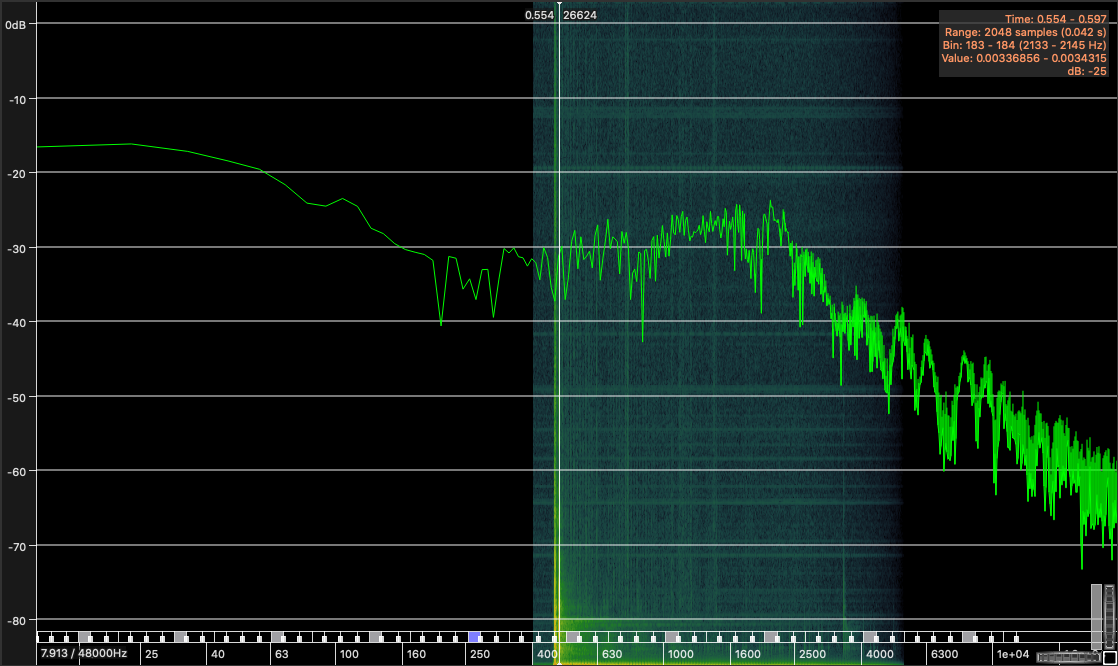
\includegraphics[width=1.\textwidth]{Unamolla_analisi_03.png}

\caption{Unamolla, Analisi n.7}

\label{fig:07_analisi_molla}

\end{center}

\end{figure}
\begin{itemize}
\item{\textbf{Analisi N. 8}: Colpo con mallet in ferro \textit{mf}.}
\item{Analisi dello spettrogramma con ascisse in frequenza.}
\item{textbf{Ripresa}: Somma segnali humb. + piezo.}
\item{textbf{Windowed}: 4096 frame.}
\end{itemize}

\begin{figure}

\begin{center}

\includegraphics[width=1.\textwidth]{Unamolla_analisi_04.png}

\caption{Unamolla, Analisi n.8}

\label{fig:08_analisi_molla}

\end{center}

\end{figure}
\begin{itemize}
\item{textbf{Analisi N. 9}: Grattato corto textit{mf}.}
\item{Analisi dello spettrogramma con ascisse in frequenza.}
\item{textbf{Ripresa}: Somma segnali humb. + piezo.}
\item{textbf{Window}: 4096 frame}
\end{itemize}

\begin{figure}

\begin{center}

\includegraphics[width=1.\textwidth]{Unamolla_analisi_05.png}

\caption{Unamolla, Analisi n.9}

\label{fig:09_analisi_molla}

\end{center}

\end{figure}
\begin{itemize}
\item{\textbf{Analisi N.10}: Grattato largo \textit{mf}.}
\item{Analisi dello spettrogramma con ascisse in frequenza.}
\item{\textbf{Ripresa}: Somma segnali humb. + piezo.}
\item{\textbf{Window}: 4096 frame.}
\end{itemize}

\begin{figure}

\begin{center}

\includegraphics[width=1.\textwidth]{Unamolla_analisi_06.png}

\caption{Unamolla, Analisi n.10}

\label{fig:10_analisi_molla}

\end{center}

\end{figure}

\begin{itemize}
\item{\textbf{Analisi N. 11}: Grattato tenuto \textit{mf}.}
\item{Analisi dello spettrogramma con ascisse in frequenza.}
\item{\textbf{Ripresa}: Somma segnali humb. + piezo.}
\item{\textbf{Windowed}: 4096 frame.}
\end{itemize}

\begin{figure}

\begin{center}

\includegraphics[width=1.\textwidth]{Unamolla_analisi_07.png}

\caption{Unamolla, Analisi n.11}

\label{fig:11_analisi_molla}

\end{center}

\end{figure}


\section*{Conclusioni}

Utilizzando mallet in ferro o l’archetto del violoncello, per quanto si risaltino un certo numero di armoniche, gli spettri rimangono con un MCD a 1. \\
Molti strumenti musicali, soprattutto nella categoria delle percussioni, hanno avuto un lungo percorso culturale prima di diventare dei veri e propri strumenti musicali. Tuttavia, non hanno avuto neppure poche modifiche e metamorfosi sia nello spettro che nell’aspetto, durante gli anni, che hanno portano a far sì che tali strumenti fossero catalogati come armonici. Grazie all’analisi, sia gestuale che spettrografica, si possono notare delle mancanze (ad esempio di una cassa di risonanza) che ha Unamolla. Di seguito vi , Grazie all’analisi si può notare che lo spettro si arricchisce di armonici se si utilizzano dei mallett in ferro o degli archetti per strumenti a corda e si fanno delle arcate corte. Così il suono è libero di propagarsi all’interno e all’esterno della molla. Inoltre, se si fa un’analisi completa dello spettro, notiamo che ci sono delle parziali, soprattutto nei casi di pizzicati e arcate corte. Se andiamo ad analizzare meglio la figura successiva, possiamo vedere come potrebbe essere eventualmente un prototipo diUnamolla 2.0 e di come sia possibile creare anche una cassa armonica variabile.
Al momento tutto ciò è solo un progetto quindi, tramite varie elaborazioni di elettronica come la creazione di filtri risonanti o di risonatori tramite micro-ritardi e feedback, possiamo arrivare ad avvicinare il suono al risultato voluto. 






% !TEX TS-program = pdflatex
% !TEX encoding = UTF-8 Unicode

%************************************************
\chapter*{Bibliografia}
\label{chp:Bibliografia}
%************************************************
\textit{Libri e articoli citati nella tesi:} \\
\\
G.A.T.M. Bollettino, a cura di Lelio Camilleri \textit{Semestrale di analisi e teoria musicale}, Anno V, Numero 1, Monografie GATM 1998, edito dal gruppo di analisi e teoria musicale, Bologna, Luglio 1998 \\
\\
A.A.V.V. a cura di Agostino di Scipio e Paolo Zavagna \textit{Musica/Tecnologia, Rivista della fondazione Ezio Franceschini}, ISSN 1974-0042, Firenze University Press, 10.2016 \\
\\
A.A.V.V. a cura di Vincenzo Santarcangelo, \textit{Have your trip, La musica di Fausto Romitelli}, Auditorium edizioni, 2014 \\
\\
Hans Bellmer, \textit{Anatomia dell’immagine} Adelphi edizioni s.p.a. Milano, 2001 \\
\\
Luciano Berio, \textit{Intervista sulla musica}, Edizioni Laterza, Bari 2011 \\
\\
Walter Branchi, \textit{Tecnologia della musica elettronica} (con prefazione di Domenico Guaccero), Lerici, Roma, 1977 \\
\\
Sergio Cingolani e Renato Spagnolo, \textit{Acustica musicale e architettonica}, UTET, Torino, 2004 \\
\\
Macdonald Critchley, \textit{Il linguaggio del gesto}, “Il pensiero Scientifico” Editore, Roma, 1979 \\
\\
Francesco Galante Nicola Sani, \textit{Musica Espansa, Percorsi elettroacustici di fine millennio}, Casa Ricordi LIM Ediitrice, 2000 \\
\\
Wassily Kandisky, \textit{Punto, linea, superficie}, Adelphi Edizioni, Roma, 1968 \\
\\
Paolo Mauri, \textit{Buio}, Casa editrice Einaudi, Trento, aprile 2007 \\
\\
Netti-Weiss, \textit{The Techniques of Saxophone Playing. Die Spieltechnik des Saxophons} \\
\\
Luigi Nono, \textit{La nostalgia del futuro, Scritti scelti 1948-1986}, Gruppo editoriale Il Saggiatore s.p.a., Milano 2007 \\
\\
Tanja Orning \textit{Pression} (a performance study) Norwegian Academy of MusicMusic Performance Research Copyright © 2012 Royal Northern College of Music Vol. 5 \\
\\
Henri Pousseur, \textit{Musica, semantica, società}, traduzione di Eugenio Costa per Casa editrice Valentino Bompiani \& C. S.p.a., Milano, 1972 \\
\\
Curtis Roads, \textit{The Computer music tutorial}, 1996 \\
\\
Simone Santi Gubini, \textit{Difettosità timbrica e subarmoniche}, Masterclass Emufest  2017, Roma \\
\\
Leonardo Scopece, \textit{Riprese Olofoniche e Ambisoniche, Il sistema 3D-VMS}, Volume quinto de LeMiniSerie, iniziativa del Centro Ricerche e Innovazione Tecnologica della RAI, settembre 2011 \\
\\
Giacinto Scelsi, \textit{Il sogno 101}, Quodlibet S.r.l., Macerata 2010 \\
\\
R. Murray Schafer, \textit{The tuning of the world}, Alfred A. Knopf, New York, 1977 \\
\\
R. Murray Schafer, \textit{Il paesaggio sonoro}, Ricordi S.r.l. e LIM Editrice S.r.l., 1985 \\
\\
Alan Stones, \textit{The Analysis of Mixed Electroacoustic Music, Kaija Saariaho's Verblendungen, a case study}
\\
Iannis Xenakis, a cura di Agostino di Scipio, \textit{Universi del suono, Scritti e interventi 1955-1994}, Ricordi S.r.l. e LIM Editrice S.r.l., 2003 \\
\\
Trevor Wishart, \textit{On Sonic Art, a new and revised edition edited by Simon Emmerson}, Published in The Netherlands by Harwood Academic Publishers, Amsterdam, 1996 \\
\\
Enore Zaffiri, \textit{Due scuole di musica elettronica in Italia} Silva Editore, Milano, 1968 \\
\\
Laura Zattra, textit{ANALYSIS AND ANALYSES OF ELECTROACOUSTIC MUSIC}, University of Padua, Department of Visual Arts and Music, Volume 36, Sound and Music Computing (SMC05), Salerno, Italy, 2005

% !TEX TS-program = pdflatex
% !TEX encoding = UTF-8 Unicode

%************************************************
\chapter*{Sitografia}
\label{chp:Sitografia}
%************************************************
\textit{Siti internet:} \\
\\
http://www.giorgionetti.com \\
\\
http://www.zavagna.it/paolo/ \\
\\
https://github.com/
\\
http://www.treccani.it
\\

% !TEX TS-program = pdflatex
% !TEX encoding = UTF-8 Unicode

%************************************************
\chapter*{Partiture}
\label{chp:Partiture}
%************************************************
\textit{Partiture e trattati utilizzati:} \\
\\
Simone Santi Gubini, \textit{Klangrelief (Relief II)} \\
\\
Giorgio Netti, \textit{Necessità di interrogare il cielo} \\
\\
Netti-Weiss, \textit{The Techniques of Saxophone Playing. Die Spieltechnik des Saxophons} \\
\\
Luigi Nono, \textit{Prometeus, Tragedia dell'ascolto}\\
\\
Fausto Romitelli, \textit{Index of metals}\\
\\
Fausto Romitelli, \textit{Professor Bad Trip, Lesson one}\\
\\
Giuseppe Silvi, \textit{pezzo per percussioni con ritardi} \\
\\

\clearpage

%!TEX TS-program = pdflatex
%!TEX encoding = UTF-8 Unicode

%*******************************************************
% Bibliography
%*******************************************************
\nocite{*}
\printbibliography

%!TEX TS-program = pdflatex
%!TEX encoding = UTF-8 Unicode
%!TEX root = ../2018-03-26-papa-vitres-de-son.tex

%*******************************************************
% Introduzione
%*******************************************************

\chapter*{Ringraziamenti}
\pdfbookmark{Ringraziamenti}{Ringraziamenti}

\textit{I più vivi ringraziamenti a tutti i colleghi ed i maestri della} \textbf{Scuola di musica elettronica} \textit{del Conservatorio di Santa Cecilia che mi hanno supportato (e sopportato), durante la stesura della tesi e del lavoro di ricerca.} \\
\\
\textit{Ringrazio Danilo Perticaro, per la viva partecipazione al progetto di ricerca.}
\\ \\
\textit{Ringrazio tutti per la partecipazione e la presenza nella mia vita, come comparse o presenze e, in qualche caso, per fortuna, assenze.} \\ \\

textit{Ringrazio tutti, un viaggio lungo, pieno di occhi e suoni meravigliosi. Un traguardo che è solo un inizio, un sogno, che diventato realtà, nella complessità della sua vita, mi fa chiudere citando uno dei miei poeti più vicini, Giacomo Leopardi:} \\
\\
\subsection*{XII - L'Infinito}
\leftskip=1cm
	\textit{Sempre caro mi fu quest'ermo colle,\\
	e questa siepe, cha da tante parte \\
	dell'ultimo orizzonte il guardo esclude. \\
	Ma sedendo e mirando, interminati \\
	spazi di l\'a da quella, e sovrumani \\
	silenzi, e profondissima quiete \\
	io nel pensier mi fingo; ove per poco \\
	il cor non si spaura. E come il vento \\
	odo stormir tra queste piante, io quello \\
	infinito silenzio a questa voce \\
	vo comparando: e mi sovvien l'eterno, \\
	e le morte stagioni, e la presente \\
	e viva, e il suon di lei. Così tra questa \\
	immensit\'a s'annega il pensier mio: \\
	e il naufragar m'è dolce in questo mare.} \\

\clearpage

		    


\clearpage

\includepdf[offset=-80 0,
		    scale=1.43,
		    pagecommand={
		    	\begin{tikzpicture}[
					remember picture,
					overlay]
		    	\node [xshift=1cm,yshift=1cm] at (current page.south west) {\color{white}{}};
				\end{tikzpicture}}
		    ]{unamolla_scritta.png}

\end{document}
